\documentclass[11pt,a4paper]{article}

\usepackage[T1]{fontenc}
\usepackage[utf8]{inputenc}
\usepackage[french]{babel}
\usepackage{lmodern}
\usepackage{textcomp}
\usepackage{graphicx}
\usepackage{array}
\usepackage{longtable}
\usepackage{booktabs}
\usepackage[a4paper,margin=2.5cm]{geometry}
\usepackage{parskip}
\usepackage{float}
\usepackage{pdflscape}
\usepackage{xcolor}
\usepackage{titlesec}
\usepackage{fancyhdr}
\usepackage{tcolorbox}
\tcbuselibrary{skins, breakable}
\usepackage{listings}
\usepackage[hidelinks]{hyperref}

% --- Caractères Unicode non couverts par inputenc, pour pdflatex ---------
\DeclareUnicodeCharacter{2264}{\ensuremath{\leq}}
\DeclareUnicodeCharacter{2265}{\ensuremath{\geq}}
\DeclareUnicodeCharacter{2260}{\ensuremath{\neq}}
\DeclareUnicodeCharacter{2192}{\ensuremath{\rightarrow}}
\DeclareUnicodeCharacter{2194}{\ensuremath{\leftrightarrow}}
\DeclareUnicodeCharacter{27F7}{\ensuremath{\longleftrightarrow}}
\DeclareUnicodeCharacter{22C8}{\ensuremath{\bowtie}}
\DeclareUnicodeCharacter{2248}{\ensuremath{\approx}}
\DeclareUnicodeCharacter{2212}{\ensuremath{-}}
\DeclareUnicodeCharacter{221D}{\ensuremath{\propto}}
\DeclareUnicodeCharacter{1D49}{\textsuperscript{e}}
\DeclareUnicodeCharacter{00B2}{\textsuperscript{2}}
\DeclareUnicodeCharacter{00B3}{\textsuperscript{3}}
\DeclareUnicodeCharacter{FFFD}{?}

% --- Couleurs (inspirées du template de la promo) ------------------------
\definecolor{agentbg}{HTML}{EFF6FF}
\definecolor{agentborder}{HTML}{3B82F6}
\definecolor{sectioncolor}{HTML}{1E3A5F}

% --- Couleurs des étiquettes de rubrique (une couleur par rubrique) -------
% Chaque rubrique d'une réponse à une question porte sa propre couleur, pour
% les repérer d'un coup d'œil au lieu d'un simple gras uniforme.
\definecolor{labrappel}{HTML}{1E3A5F}    % bleu nuit  — l'énoncé
\definecolor{labfichier}{HTML}{6D28D9}   % violet     — le code Python
\definecolor{labverif}{HTML}{0A7B34}     % vert       — la vérification pandas
\definecolor{labresultat}{HTML}{B45309}  % ambre      — le résultat / la sortie
\definecolor{labanalyse}{HTML}{0E7490}   % teal       — l'analyse manuelle
\definecolor{labcomment}{HTML}{475569}   % gris ardoise — la synthèse
% Étiquette de rubrique : gras + couleur dédiée.
\newcommand{\rub}[2]{\textbf{\textcolor{#1}{#2}}}

% --- Boîte « Travail avec l'agent » --------------------------------------
% Équivalent visuel des boîtes « Prompt » du template : ici le travail
% n'a pas reposé sur des prompts copiables mais sur l'agent Claude Code,
% d'où le titre de la boîte.
\newtcolorbox{agentbox}{
  breakable, enhanced,
  colback=agentbg, colframe=agentborder,
  boxrule=1.2pt, arc=4pt,
  left=10pt, right=10pt, top=8pt, bottom=8pt,
  title={\textbf{\textsf{Travail avec l'agent --- Claude Code}}},
  fonttitle=\color{white}\bfseries\small,
  attach boxed title to top left={yshift=-2mm, xshift=6mm},
  boxed title style={colback=agentborder, arc=3pt, boxrule=0pt},
}

% --- Bloc « vérification pandas » (style notebook : code + sortie df) -----
\definecolor{pyblockbg}{HTML}{F6F8FA}
\definecolor{pyblockframe}{HTML}{D0D7DE}
\definecolor{pykw}{HTML}{1E3A5F}
\definecolor{pycomment}{HTML}{6A737D}
\definecolor{pystr}{HTML}{0A7B34}
\lstdefinestyle{pyblock}{
  language=Python,
  basicstyle=\ttfamily\footnotesize,
  backgroundcolor=\color{pyblockbg},
  frame=single, framerule=0.6pt, rulecolor=\color{pyblockframe},
  keywordstyle=\color{pykw}\bfseries,
  commentstyle=\color{pycomment}\itshape,
  stringstyle=\color{pystr},
  showstringspaces=false, breaklines=true, columns=fullflexible,
  xleftmargin=6pt, xrightmargin=6pt, aboveskip=6pt, belowskip=8pt,
  extendedchars=true,
  literate={é}{{\'e}}1 {è}{{\`e}}1 {ê}{{\^e}}1 {à}{{\`a}}1 {â}{{\^a}}1
           {ç}{{\c c}}1 {î}{{\^\i}}1 {ï}{{\"\i}}1 {ô}{{\^o}}1 {û}{{\^u}}1
           {É}{{\'E}}1 {È}{{\`E}}1 {→}{{$\rightarrow$}}1 {×}{{$\times$}}1
           {’}{{'}}1 {…}{{...}}3,
}

% --- Titres colorés ------------------------------------------------------
\titleformat{\section}{\color{sectioncolor}\Large\bfseries}{\thesection}{1em}{}
\titleformat{\subsection}{\color{sectioncolor}\large\bfseries}{\thesubsection}{1em}{}
\titleformat{\subsubsection}{\color{sectioncolor}\normalsize\bfseries}{\thesubsubsection}{1em}{}

% --- En-têtes et pieds de page -------------------------------------------
\pagestyle{fancy}
\fancyhf{}
\fancyhead[L]{Accidents de la route}
\fancyhead[R]{Projet Data}
\fancyfoot[C]{\thepage}
\renewcommand{\headrulewidth}{0.4pt}
\setlength{\headheight}{14pt}

\begin{document}

% ============================================================================
% PAGE DE TITRE
% ============================================================================
\begin{titlepage}
\centering
\IfFileExists{logo_sorbonne.png}{
\includegraphics[width=0.30\textwidth]{logo_sorbonne.png}\\[1cm]}{\vspace*{1cm}}
{\scshape\LARGE Université Paris 1 --- Panthéon-Sorbonne}\\[0.5cm]
{\scshape\Large Master MIMO}\\[1.5cm]
\rule{\linewidth}{0.5mm}\\[0.4cm]
{\huge\bfseries Projet Data en Python\\[0.4cm]}
\rule{\linewidth}{0.5mm}\\[1.5cm]
{\Large\textbf{Analyse du fichier BAAC --- accidents de la route 2005--2015}}\\[3cm]
\begin{minipage}{0.4\textwidth}
\begin{flushleft}\large
\emph{Présenté par :}\\
\textbf{Rayan Leveque}\\
\textbf{Tom Séguier}
\end{flushleft}
\end{minipage}
\begin{minipage}{0.4\textwidth}
\begin{flushright}\large
\emph{Sous la direction de :}\\
\textbf{M. Grosz}\\
\textbf{M. Giron}
\end{flushright}
\end{minipage}\\[3cm]
\vfill
{\large Année universitaire 2025--2026}
\end{titlepage}

\section*{En-tête}
\addcontentsline{toc}{section}{En-tête}

\begin{itemize}
\item \textbf{Membres du groupe} : Rayan Leveque, Tom Séguier
\item \textbf{Période étudiée} : 2005 – 2015 inclus (Groupe 1, 11 années)
\item \textbf{Outil d'IA générative utilisé} : \textbf{Claude Code} (Anthropic), modèle Claude Opus 4.7 (1M context)
\end{itemize}

\subsection*{Note sur l'usage de l'outil}
\addcontentsline{toc}{subsection}{Note sur l'usage de l'outil}

Claude Code est un \textbf{agent IA conversationnel} doté d'outils (lecture/écriture de fichiers, exécution de commandes shell, etc.), et non un LLM one-shot type ChatGPT. Le workflow n'a donc pas reposé sur des prompts uniques copiables, mais sur une \textbf{conversation itérative} avec l'agent, intégrée à l'environnement de développement (terminal).

En conséquence, la rubrique "prompt utilisé" du barème de référence (§1.4.1 du sujet) est remplacée dans ce dossier par une rubrique \textbf{"Travail avec l'agent"}, qui décrit pour chaque question :

\begin{itemize}
\item Le \textbf{contexte donné à l'agent} : contraintes, données d'entrée, format de sortie attendu.
\item Les \textbf{itérations et décisions} : ce qui a été ajusté, ce qui a posé problème, ce qui a été validé.
\end{itemize}

Cette approche est honnête sur le workflow réel, et l'analyse de la stratégie d'usage d'un agent IA (vs prompting one-shot) est développée dans l'exposé.

\tableofcontents
\newpage

\section*{1. Récupération et formatage des données}
\addcontentsline{toc}{section}{1. Récupération et formatage des données}

\clearpage
\subsection*{Question 0.0 — Téléchargement des données BAAC}
\addcontentsline{toc}{subsection}{Question 0.0 — Téléchargement des données BAAC}

\rub{labrappel}{Rappel de la question :} récupérer les fichiers caracteristiques, lieux, vehicules, usagers pour les années 2005–2015, depuis \href{https://www.data.gouv.fr/fr/datasets/base-de-donnees-accidents-corporels-de-la-circulation/}{data.gouv.fr}, ainsi que le PDF de description des bases.

\begin{agentbox}
\begin{itemize}
\item \textbf{Contexte} : automatiser le téléchargement plutôt que de cliquer 45 fois sur des liens, en s'assurant d'exclure les \texttt{vehicules-immatricules-baac…} (piège du sujet).
\item \textbf{Itérations} : première version basée sur les titres des ressources de l'API data.gouv.fr ; le filtre ratait \texttt{caracteristiques} à cause des accents (titres en \texttt{caractéristiques}), corrigé en normalisant via \texttt{unicodedata} et en matchant aussi le nom de fichier de l'URL.
\end{itemize}
\end{agentbox}

\rub{labfichier}{Fichier Python :} \texttt{python/download\_data.py} \emph{(hors barème — script utilitaire de setup, pas une réponse à une question notée)}.

\rub{labresultat}{Résultat :} \textasciitilde{}44 fichiers CSV + 1 PDF déposés dans \texttt{data/raw/}.

\rub{labanalyse}{Vérifications.} \texttt{ls data/raw/ | wc -l} confirme le compte attendu (4 types × 11 ans + 1 PDF). Échantillonnage manuel : ouverture de 2-3 CSV pour confirmer qu'ils correspondent bien au type annoncé.

\clearpage
\subsection*{Question 1.1 — Conversion UTF-8, séparateur \texttt{,}}
\addcontentsline{toc}{subsection}{Question 1.1 — Conversion UTF-8, séparateur \texttt{,}}

\rub{labrappel}{Rappel de la question.} Par précaution, transformer le codage de tous les fichiers de données au format UTF-8 et s'assurer que le séparateur est bien \texttt{,}.

\begin{agentbox}
\begin{itemize}
\item \textbf{Contexte} : 44 fichiers \texttt{data/raw/} → \texttt{data/utf8/} (nommage \texttt{\{type\}\_\{année\}.csv}), code en français.
\item \textbf{Décision} : détection automatique de l'encodage (\texttt{chardet}) \emph{et} du séparateur plutôt qu'une conversion UTF-8 en dur ; relecture/réécriture via \texttt{csv.reader}/\texttt{csv.writer} pour un quoting propre.
\item \textbf{Itération} : l'inspection manuelle préalable (\texttt{file}, \texttt{od -c}) a révélé \texttt{caracteristiques\_2009.csv} en séparateur tabulation — c'est ce cas qui justifie la détection automatique du séparateur.
\end{itemize}
\end{agentbox}

\rub{labfichier}{Fichier Python :} \texttt{python/question11.py}.

\rub{labverif}{Vérification (pandas)} --- \texttt{python/verification11.py} → \texttt{results/verification11.txt} :

\begin{lstlisting}[style=pyblock]
>>> for f in utf8.glob("*.csv"):          # 44 fichiers
...     f.read_bytes().decode("utf-8")      # decode UTF-8 OK
...     pd.read_csv(f, sep=",").shape[1]     # == nb colonnes attendu
>>> recap

            type  fichiers  utf8+sep_ok
caracteristiques        11           11
           lieux        11           11
       vehicules        11           11
         usagers        11           11

# conforme : 44/44 fichiers UTF-8, sep ',', bon nb de colonnes
\end{lstlisting}

\rub{labresultat}{Résultat :} \texttt{results/reponse11.txt} (44 fichiers convertis, 0 manquant). Synthèse des encodages détectés : 34 fichiers déjà en UTF-8 (lieux, vehicules, usagers de toutes années), 9 fichiers en \texttt{iso-8859-1} (caracteristiques 2005, 2007–2015), 1 fichier en \texttt{windows-1252} (caracteristiques 2006). Séparateurs : 43 fichiers en \texttt{,}, 1 fichier en tabulation (caracteristiques 2009).

\rub{labanalyse}{Vérifications.}

\begin{itemize}
\item \emph{Comptes de lignes} : \texttt{wc -l} sur les fichiers source et cible donne le même résultat pour chaque fichier (ex. 87 027 lignes pour \texttt{caracteristiques\_2005.csv} source et cible) — preuve qu'aucune ligne n'a été perdue.
\item \emph{Encodage} : \texttt{file data/utf8/caracteristiques\_2009.csv} renvoie \texttt{CSV Unicode text, UTF-8 text} (idem pour les fichiers initialement en latin-1).
\item \emph{Caractères accentués} : \texttt{grep -E "É|é|è|ç"} sur \texttt{caracteristiques\_2005.csv} (ex-\texttt{iso-8859-1}) renvoie des libellés correctement décodés (\texttt{Théodore Blot}, \texttt{libération}, \texttt{intermarché}).
\item \emph{Cas 2009} : le fichier source contenait déjà des caractères de remplacement Unicode (\texttt{U+FFFD}, vus comme \texttt{�}) provenant d'une corruption en amont chez le producteur des données — la conversion les conserve à l'identique, on ne peut pas les reconstruire ; cela sera signalé comme une limite des données dans la conclusion.
\item \emph{Quoting CSV} : le passage par \texttt{csv.writer} garantit que si un champ contient \texttt{,}, il sera entouré de guillemets — c'est plus robuste qu'un simple \texttt{replace('\textbackslash{}\textbackslash{}t', ',')}.
\end{itemize}

\rub{labcomment}{Commentaires.} La diversité d'encodages (3 encodages distincts) et le séparateur tabulation isolé en 2009 confirment que la précaution demandée par l'énoncé est nécessaire : sans cette étape, un script Q2+ qui lirait \texttt{caracteristiques\_2009.csv} en supposant \texttt{utf-8 + ,} casserait silencieusement (lignes considérées comme une seule colonne).

\clearpage
\subsection*{Question 1.2 — Vérification de structure et tableaux récapitulatifs}
\addcontentsline{toc}{subsection}{Question 1.2 — Vérification de structure et tableaux récapitulatifs}

\rub{labrappel}{Rappel de la question.} Vérifier par programme que pour chaque type de fichier (caractéristiques, lieux, véhicules, usagers), les fichiers des différentes années ont une structure conforme à la documentation. Produire 4 tableaux récapitulatifs avec le nombre de lignes par année et le cumul pour chaque type.

\begin{agentbox}
\begin{itemize}
\item \textbf{Contexte} : entrée \texttt{data/utf8/}, schéma de référence par type tiré de la doc BAAC et des en-têtes 2005-2015 (caracteristiques 16 colonnes, lieux 18, vehicules 9, usagers 12).
\item \textbf{Choix} : comptage \texttt{csv.reader} ligne à ligne (plus pédagogique que \texttt{pandas} pour la soutenance), comparaison des en-têtes par ensemble \emph{et} par ordre — pour distinguer colonne manquante, colonne inattendue et ordre incorrect.
\item \textbf{Itération} : inspection préalable des 44 en-têtes (\texttt{head -1}) confirmant un schéma stable sur la période, d'où un schéma unique par type plutôt que par (type, année).
\end{itemize}
\end{agentbox}

\rub{labfichier}{Fichier Python :} \texttt{python/question12.py}.

\rub{labverif}{Vérification (pandas)} --- \texttt{python/verification12.py} → \texttt{results/verification12.txt} :

\begin{lstlisting}[style=pyblock]
>>> df = pd.read_csv(f, dtype=str)
>>> list(df.columns) == schema_attendu      # en-tete exact ?
>>> recap                                    # nb de lignes par type

            type  colonnes schema_ok  total_lignes
caracteristiques        16     11/11        780553
           lieux        18     11/11        780553
       vehicules         9     11/11       1331465
         usagers        12     11/11       1742583

# conforme : en-tete exact (colonnes+ordre) pour les 44 fichiers
\end{lstlisting}

\rub{labresultat}{Résultat :} \texttt{results/reponse12.txt}. Cumul par type pour 2005-2015 : caracteristiques \textbf{780 553}, lieux \textbf{780 553} (cohérent avec caracteristiques — 1 ligne lieu par accident), vehicules \textbf{1 331 465}, usagers \textbf{1 742 583}. Cumul global : \textbf{4 635 154 lignes} de données. Aucun écart de schéma : les 44 fichiers ont exactement les colonnes attendues, dans le bon ordre.

\rub{labanalyse}{Vérifications.}

\begin{itemize}
\item \emph{Cohérence avec Q1.1} : Q1.1 comptait \texttt{nb\_lignes} en incluant l'en-tête (87 027 pour \texttt{caracteristiques\_2005.csv}), Q1.2 compte les lignes de données seules (87 026). L'écart constant de 1 ligne par fichier confirme qu'aucune ligne de données n'a été perdue lors de la conversion UTF-8.
\item \emph{Égalité caracteristiques ↔ lieux par année} : pour chaque année, le nombre de lignes de \texttt{caracteristiques} est strictement égal à celui de \texttt{lieux} (87 026 = 87 026 en 2005, etc.) — première vérification de la relation 1-pour-1 entre un accident et son lieu, qui sera approfondie en Q2.4.
\item \emph{Ratios} : le ratio \texttt{usagers / caracteristiques} est de 2,23 sur la période (4 635 154 / 780 553 → en moyenne ≈ 2,23 usagers par accident), et \texttt{vehicules / caracteristiques} ≈ 1,71 — ordres de grandeur plausibles pour des accidents de la circulation, où la majorité implique 2 véhicules.
\item \emph{Schéma stable sur 11 ans} : aucune colonne ajoutée ou retirée entre 2005 et 2015 pour les 4 types — la doc BAAC dont on s'est servi décrit donc bien la totalité du périmètre du Groupe 1.
\end{itemize}

\rub{labcomment}{Commentaires.} L'absence d'écart de schéma est une bonne nouvelle pour la suite : les scripts Q2+ pourront supposer un en-tête fixe par type. À noter que la baisse du nombre d'accidents sur la période (87 k en 2005 → 58 k en 2015, soit −33 \%) est visible directement dans le cumul des \texttt{caracteristiques} ; c'est cohérent avec la tendance nationale connue de baisse de l'accidentologie routière, et cela sera repris en Q6.1 (analyse temporelle).

\clearpage
\subsection*{Question 1.3 — Enrichissement avec libellés des domaines énumérés}
\addcontentsline{toc}{subsection}{Question 1.3 — Enrichissement avec libellés des domaines énumérés}

\rub{labrappel}{Rappel de la question.} Pour tous les fichiers obtenus en 1.1, générer une nouvelle version où toutes les valeurs des domaines énumérés sont complétées avec le libellé correspondant (ex. \texttt{1} pour \texttt{lum} devient \texttt{1 - Plein jour}). Vérifier la transformation, en portant une attention particulière à \texttt{catv} (catégorie de véhicule).

\begin{agentbox}
\begin{itemize}
\item \textbf{Contexte} : 26 colonnes énumérées sur les 4 types, sortie \texttt{data/enriched/} au format \texttt{code - libellé}, libellés tirés de la doc PDF ONISR 2005-2018 et de \texttt{docs/schema\_baac.md}.
\item \textbf{Implémentation} : un dictionnaire par colonne (code → libellé), dispatch \texttt{MAPPINGS[type][colonne]}, parcours \texttt{csv.reader}/\texttt{csv.writer} ligne à ligne.
\item \textbf{Itération clé} : les codes \texttt{catv}, \texttt{obs}, \texttt{manv} sont zero-paddés sur 2 chiffres (\texttt{07}, \texttt{01}, \texttt{30}…), d'où l'ajout d'un \texttt{normaliser\_code()} (\texttt{zfill(2)}) avant lookup. Décision validée : ne \textbf{pas} enrichir les valeurs absentes (\texttt{''}, \texttt{'.'}, \texttt{-1}) ni les codes hors mapping — conservés bruts pour l'analyse en Q4.
\end{itemize}
\end{agentbox}

\rub{labfichier}{Fichier Python :} \texttt{python/question13.py}.

\rub{labverif}{Vérification (pandas)} --- \texttt{python/verification13.py} → \texttt{results/verification13.txt} :

\begin{lstlisting}[style=pyblock]
>>> ok = col.str.contains(" - ") | col.isin(MARQUEURS)  # enrichi/absent
>>> recap                                    # lignes conservees + hors mapping

            type  lignes_utf8  lignes_enriched  hors_mapping
caracteristiques       780553           780553             0
           lieux       780553           780553             0
       vehicules      1331465          1331465             0
         usagers      1742583          1742583             0

# conforme : aucune ligne perdue, 0 valeur hors mapping, catv 33 libelles
\end{lstlisting}

\rub{labresultat}{Résultat :} 44 fichiers enrichis dans \texttt{data/enriched/} (rapport détaillé dans \texttt{results/reponse13.txt}). Cumul sur 2005-2015 : \textasciitilde{}21,4 millions de cellules enrichies. Sur la colonne \textbf{\texttt{catv}} (1 331 465 lignes véhicules), \textbf{100 \% des codes rencontrés sont répertoriés} (33 codes distincts, du plus fréquent \texttt{07 - VL seul} à 825 576 occurrences au plus rare \texttt{11 - VU + caravane} à 17 occurrences). Aucun code \texttt{catv} n'est donc orphelin du mapping — le piège mentionné dans le sujet est neutralisé.

\rub{labanalyse}{Vérifications.}

\begin{itemize}
\item \emph{Comptage de lignes} : \texttt{wc -l} sur source vs cible donne le même résultat (ex. 69 380 lignes pour \texttt{caracteristiques\_2010.csv} source et cible) — aucune ligne perdue.
\item \emph{Couverture \texttt{catv}} : la rubrique "4. Vérification ciblée" du rapport balaye les 11 années de \texttt{vehicules\_*.csv} enrichis et confirme que les 33 codes rencontrés sont tous étiquetés \texttt{enrichi} (aucun \texttt{non répertorié}).
\item \emph{Inspection visuelle} : \texttt{head -3 data/enriched/\{caracteristiques,lieux,vehicules,usagers\}\_2010.csv} montre des libellés propres (ex. \texttt{1 - Plein jour}, \texttt{30 - Scooter ≤ 50 cm³}, \texttt{0 - Sans objet}).
\item \emph{Colonnes non-énumérées préservées} : \texttt{Num\_Acc}, \texttt{dep}, \texttt{voie}, \texttt{secu}, \texttt{an\_nais}, etc. apparaissent inchangées dans les fichiers enrichis — la transformation est strictement ciblée.
\item \emph{Cellules "hors mapping"} : 1,67 M cellules au total (essentiellement \texttt{senc=0} pour les 2 années où le sens de circulation est non renseigné, \texttt{manv=00}, et \texttt{circ/prof/plan/surf/situ=0} dans \texttt{lieux}). Toutes correspondent au code \texttt{0} non documenté dans la doc PDF mais utilisé en pratique comme marqueur "non renseigné". Décision : on les laisse à \texttt{0} brut. Cela sera repris en Q4 (où on les compte comme absentes) et en Q5 (où elles n'interfèrent pas avec les contrôles d'incohérence).
\end{itemize}

\rub{labcomment}{Commentaires.} L'enrichissement remplit deux rôles : (1) rendre les fichiers \texttt{data/enriched/} directement lisibles par un humain (utile en debug et pour générer les tableaux narratifs des questions ultérieures), (2) servir de base unique aux Q2-Q6 — toutes ces questions liront depuis \texttt{data/enriched/} plutôt que \texttt{data/utf8/}, ce qui garantit que les répartitions calculées en Q3.1 et les vérifications de cohérence en Q5 utiliseront exactement les mêmes libellés que ceux qui apparaîtront dans le rapport. Le format \texttt{code - libellé} (plutôt que le libellé seul) préserve la possibilité de retrier ou regrouper sur le code numérique d'origine si nécessaire — c'est moins coûteux que de re-décoder en sens inverse.

\section*{2. Étude de la qualité des données}
\addcontentsline{toc}{section}{2. Étude de la qualité des données}

\subsection*{2.1. Intégrité référentielle}
\addcontentsline{toc}{subsection}{2.1. Intégrité référentielle}

\clearpage
\subsubsection*{Question 2.1 — Usager → Véhicule}
\addcontentsline{toc}{subsubsection}{Question 2.1 — Usager → Véhicule}

\rub{labrappel}{Rappel de la question.} Vérifier par programme que chaque usager fait référence à un véhicule présent dans les véhicules. Les données incohérentes doivent être listées dans un fichier dédié, analysées et commentées.

\begin{agentbox}
\begin{itemize}
\item \textbf{Contexte} : entrée \texttt{data/enriched/}, clé de jointure \texttt{(Num\_Acc, num\_veh)} — un usager pointe vers son véhicule (conducteur/passager) ou celui qui l'a heurté (piéton).
\item \textbf{Choix} : traitement année par année — les couples \texttt{(Num\_Acc, num\_veh)} de \texttt{vehicules} chargés dans un \texttt{set} Python (test d'appartenance en O(1)), puis parcours de \texttt{usagers} ligne à ligne.
\item \textbf{Itération} : inspection préalable des en-têtes (\texttt{head -1}) confirmant que \texttt{num\_veh} existe des deux côtés — jointure directe sans renommage.
\end{itemize}
\end{agentbox}

\rub{labfichier}{Fichier Python :} \texttt{python/question21.py}.

\rub{labverif}{Vérification (pandas)} --- \texttt{python/verification21.py} → \texttt{results/verification21.txt} :

\begin{lstlisting}[style=pyblock]
>>> f = usagers.merge(vehicules, on=["Num_Acc","num_veh"],
...                    how="left", indicator=True)
>>> recap          # violations = lignes "left_only" par annee

 annee  usagers  couples_veh  violations
  2005   197498       149764           2
  2006   187085       142300           5
  2007   188457       144130          11
  2008   170960       131048           4
  2009   165962       126347           0
  2010   154192       117743           0
  2011   148543       113854           0
  2012   138628       105814           0
  2013   128694        98925           0
  2014   132186       101762           0
  2015   130378        99778           0

# conforme : 22 violations / 13 couples distincts (identique a reponse21_violations.csv)
\end{lstlisting}

\rub{labresultat}{Résultat :} \texttt{results/reponse21.txt} + \texttt{results/reponse21\_violations.csv}. Sur \textbf{1 742 583 usagers} cumulés sur 2005-2015, \textbf{22 violations} détectées, soit \textbf{0,0013 \%} — toutes concentrées sur 2005-2008 (2, 5, 11, 4 violations respectivement) ; \textbf{à partir de 2009 l'intégrité est parfaite} (0 violation chaque année). Aucune violation n'est dûe à un \texttt{num\_veh} vide : il s'agit à chaque fois d'un identifiant non vide pointant vers un véhicule inexistant pour le \texttt{Num\_Acc} concerné.

\rub{labanalyse}{Vérifications.}

\begin{itemize}
\item \emph{Cohérence des totaux} : la somme des \texttt{nb\_usagers} par année (1 742 583) coïncide exactement avec le cumul calculé en Q1.2 — preuve que toutes les lignes sont bien balayées.
\item \emph{Inspection manuelle de violations} : sur l'accident 200500086196 (2005), le fichier \texttt{vehicules} n'enregistre que \texttt{A01} et \texttt{B02}, mais un piéton est saisi avec \texttt{num\_veh=A03} — le saisisseur a probablement noté la lettre du véhicule heurtant sans vérifier l'enregistrement côté véhicules. Sur 200700083469 (2007), le fichier vehicules contient \texttt{A01} (VL) et \texttt{B01} (autobus) ; les 9 passagers du bus sont ventilés entre \texttt{B01} et \texttt{B02}, alors qu'aucun véhicule \texttt{B02} n'a été déclaré — visiblement, le saisisseur a inventé un second véhicule pour répartir les passagers. Ces deux exemples confirment l'origine \emph{humaine} (saisie BAAC sur procès-verbal) des erreurs.
\item \emph{Réciprocité non-implicite} : ce contrôle ne dit rien des véhicules sans usager (cas inverse) — c'est l'objet de Q2.2.
\item \emph{Échantillon vs exhaustif} : le fichier CSV contient bien les 22 violations (\texttt{wc -l reponse21\_violations.csv} = 23 = 22 + en-tête).
\end{itemize}

\rub{labcomment}{Commentaires.} Le taux de violations (0,0013 \%) est négligeable et ne biaise aucune analyse statistique ultérieure. La concentration sur 2005-2008 puis disparition totale à partir de 2009 suggère soit un durcissement du contrôle d'intégrité dans la chaîne de saisie BAAC autour de 2008-2009, soit un nettoyage rétroactif partiel des fichiers récents. Les violations restantes seront simplement ignorées dans les questions suivantes ; la liste exhaustive reste disponible dans \texttt{reponse21\_violations.csv} pour qui voudrait les exclure explicitement par jointure.

\clearpage
\subsubsection*{Question 2.2 — Véhicule → ≥ 1 Usager}
\addcontentsline{toc}{subsubsection}{Question 2.2 — Véhicule → ≥ 1 Usager}

\rub{labrappel}{Rappel de la question.} Vérifier par programme que chaque véhicule décrit dans les véhicules est associé à au moins un usager. Si des données incohérentes existent, elles doivent être toutes listées dans un fichier dédié, analysées et commentées.

\begin{agentbox}
\begin{itemize}
\item \textbf{Contexte} : contrôle réciproque de Q2.1 — même clé \texttt{(Num\_Acc, num\_veh)}, sens inversé (on parcourt \texttt{vehicules}, on vérifie l'existence côté \texttt{usagers}).
\item \textbf{Choix} : structure miroir de \texttt{question21.py} — les couples \texttt{usagers} dans un \texttt{set}, puis parcours de \texttt{vehicules}.
\item \textbf{Itération} : validation manuelle de la cause supposée sur le 1\textsuperscript{er} cas (accident \texttt{200500000170}) — un VU \texttt{B02} sans aucun usager rattaché, signature d'une fuite ; l'analyse nomme explicitement ce scénario plutôt que de parler vaguement d'« erreurs de saisie ».
\end{itemize}
\end{agentbox}

\rub{labfichier}{Fichier Python :} \texttt{python/question22.py}.

\rub{labverif}{Vérification (pandas)} --- \texttt{python/verification22.py} → \texttt{results/verification22.txt} :

\begin{lstlisting}[style=pyblock]
>>> f = vehicules.merge(usagers, on=["Num_Acc","num_veh"],
...                      how="left", indicator=True)
>>> recap          # vehicules sans usager par annee

 annee  vehicules  couples_usa  violations
  2005     149764       147779        1987
  2006     142300       140264        2040
  2007     144130       141975        2158
  2008     131048       129052        2000
  2009     126347       124708        1639
  2010     117743       116141        1602
  2011     113854       112211        1643
  2012     105814       104217        1597
  2013      98925        97348        1577
  2014     101762       100063        1699
  2015      99778        98140        1638

# conforme : 19 580 vehicules sans usager (identique)
\end{lstlisting}

\rub{labresultat}{Résultat :} \texttt{results/reponse22.txt} + \texttt{results/reponse22\_violations.csv}. Sur \textbf{1 331 465 véhicules} cumulés sur 2005-2015, \textbf{19 580 véhicules sans usager} (1,4706 \%), répartis de manière régulière sur toute la période (1577 à 2158 par année, sans rupture franche entre les années anciennes et récentes — contrairement à Q2.1). Aucun \texttt{num\_veh} vide côté véhicules : la clé est toujours bien renseignée, le problème ne vient pas de la saisie de l'identifiant mais bien de l'absence d'un usager rattaché.

\rub{labanalyse}{Vérifications.}

\begin{itemize}
\item \emph{Cohérence des totaux} : la somme des \texttt{nb\_vehicules} (1 331 465) coïncide exactement avec le cumul \texttt{vehicules} calculé en Q1.2 — preuve que toutes les lignes sont bien balayées.
\item \emph{Inspection manuelle d'un cas} : sur l'accident \texttt{200500000170} (2005), \texttt{vehicules} enregistre \texttt{A01} (bicyclette) et \texttt{B02} (VU 1,5T-3,5T) ; côté \texttt{usagers}, seul le cycliste (\texttt{A01}, blessé léger, conducteur) est saisi — aucun usager pour le VU \texttt{B02}. Sans information sur le conducteur du VU, le scénario le plus crédible est une fuite après collision avec le cycliste, où le véhicule a été identifié (par le cycliste, des témoins, ou la plaque) sans que son conducteur ne soit retrouvé au moment du PV. Cela colle au cas connu signalé dans l'énoncé du sujet.
\item \emph{Stationnarité dans le temps} : contrairement à Q2.1 (concentration sur 2005-2008), le taux ici est stable sur 11 ans (\textasciitilde{}1,5 \% chaque année, taux le plus bas en 2013 = 1,59 \%, le plus haut en 2007 = 1,50 \%). Ce profil "bruit de fond constant" est cohérent avec un phénomène structurel (fuites de conducteurs) et non avec une erreur de saisie ponctuelle qui aurait été corrigée — preuve indirecte supplémentaire de l'interprétation "fuite".
\item \emph{Réciprocité} : le contrôle Q2.1 portait sur \texttt{usagers → vehicules} (22 violations) ; ici c'est l'inverse \texttt{vehicules → usagers} (19 580 violations). Les deux ne couvrent pas le même problème — Q2.1 attrape les usagers fantômes (saisie incorrecte du \texttt{num\_veh}), Q2.2 attrape les véhicules fantômes (conducteur absent du PV).
\end{itemize}

\rub{labcomment}{Commentaires.} Les 19 580 violations ne sont \textbf{pas} des erreurs de qualité à supprimer : elles portent une information réelle (un véhicule a été impliqué dans l'accident, mais son conducteur n'a pas pu être identifié). Cette interprétation est confirmée à la fois par l'inspection manuelle du premier cas et par la stationnarité temporelle du taux. Décision pour la suite : ces véhicules restent comptabilisés dans toutes les analyses centrées sur les véhicules (Q3.1 sur les attributs énumérés \texttt{vehicules}, Q4.1 sur les valeurs absentes véhicules, Q6 si répartition par catégorie de véhicule), mais ils n'apparaîtront évidemment pas dans les analyses centrées sur les usagers (gravité, âge, sexe, sécurité). À noter que ce ratio (\textasciitilde{}1,5 \% de véhicules sans conducteur identifié) est lui-même un indicateur intéressant pour la conclusion : la base BAAC capture ainsi indirectement le taux de délit de fuite.

\clearpage
\subsubsection*{Question 2.3 \emph{(facultative)} — Lieu → Accident}
\addcontentsline{toc}{subsubsection}{Question 2.3 \emph{(facultative)} — Lieu → Accident}

\rub{labrappel}{Rappel de la question.} Vérifier par programme que chaque lieu fait référence à un accident présent dans les caractéristiques. Si des données incohérentes existent, elles doivent être toutes listées dans un fichier dédié, analysées et commentées.

\begin{agentbox}
\begin{itemize}
\item \textbf{Contexte} : intégrité référentielle sur la clé \texttt{Num\_Acc} seule — chaque ligne de \texttt{lieux} doit pointer vers un accident présent dans \texttt{caracteristiques}.
\item \textbf{Choix} : miroir de \texttt{question22.py} — les \texttt{Num\_Acc} de \texttt{caracteristiques} dans un \texttt{set}, puis parcours de \texttt{lieux}.
\item \textbf{Itération} : sous-décompte « dont \texttt{Num\_Acc} vide » (resté à 0) pour distinguer une clé manquante d'une vraie référence cassée.
\end{itemize}
\end{agentbox}

\rub{labfichier}{Fichier Python :} \texttt{python/question23.py}.

\rub{labverif}{Vérification (pandas)} --- \texttt{python/verification23.py} → \texttt{results/verification23.txt} :

\begin{lstlisting}[style=pyblock]
>>> f = lieux.merge(caracteristiques, on="Num_Acc",
...                  how="left", indicator=True)
>>> recap          # lieux orphelins par annee

 annee  lieux  accidents  violations
  2005  87026      87026           0
  2006  82993      82993           0
  2007  83850      83850           0
  2008  76767      76767           0
  2009  74409      74409           0
  2010  69379      69379           0
  2011  66974      66974           0
  2012  62250      62250           0
  2013  58397      58397           0
  2014  59854      59854           0
  2015  58654      58654           0

# conforme : 0 lieu orphelin (identique)
\end{lstlisting}

\rub{labresultat}{Résultat :} \texttt{results/reponse23.txt} + \texttt{results/reponse23\_violations.csv}. Sur \textbf{780 553 lieux} cumulés sur 2005-2015, \textbf{0 violation} (0,0000 \%) : chaque lieu référence un accident existant. Fait notable révélé par le récapitulatif : pour \textbf{chaque} année, le nombre de lieux est \textbf{strictement égal} au nombre d'accidents distincts (87 026 = 87 026 en 2005, …, 58 654 = 58 654 en 2015). Le fichier \texttt{reponse23\_violations.csv} ne contient que son en-tête.

\rub{labanalyse}{Vérifications.}

\begin{itemize}
\item \emph{Égalité lieux = accidents} : l'identité parfaite entre \texttt{nb\_lieux} et \texttt{nb\_accidents} chaque année est un signal fort — non seulement chaque lieu pointe vers un accident existant (le contrôle demandé), mais il y a \textbf{exactement un lieu par accident}. Cela préfigure le résultat de Q2.4 (relation 1-à-1 accident → lieu) et sera confirmé dans ce sens-là.
\item \emph{Cohérence des totaux} : la somme des \texttt{nb\_lieux} (780 553) coïncide avec le cumul \texttt{lieux} calculé en Q1.2 — toutes les lignes sont bien balayées.
\item \emph{Sous-décompte \texttt{Num\_Acc} vide} : 0 cas, donc aucune violation « factice » dûe à une clé manquante — le résultat de 0 violation est un vrai 0, pas un artefact de clés vides qui se seraient retrouvées dans le set.
\item \emph{Fichier exhaustif} : \texttt{wc -l reponse23\_violations.csv} = 1 (en-tête seul), cohérent avec 0 violation.
\end{itemize}

\rub{labcomment}{Commentaires.} Le résultat est celui attendu par le modèle de données BAAC : le fichier \texttt{lieux} décrit la voirie de l'accident à raison d'une ligne par \texttt{Num\_Acc}, en relation 1-à-1 avec \texttt{caracteristiques}. Contrairement à Q2.2 (où les véhicules « fantômes » portaient une information réelle de fuite), il n'y a ici aucune anomalie à interpréter : l'intégrité est parfaite et aucune donnée n'est à exclure pour la suite. L'égalité observée \texttt{lieux = accidents} chaque année est l'apport principal de cette question — elle garantit aux analyses spatiales ultérieures (Q6 cartographie, Q3 attributs de voirie) qu'une jointure \texttt{caracteristiques ⋈ lieux} sur \texttt{Num\_Acc} ne créera ni perte ni duplication de lignes.

\clearpage
\subsubsection*{Question 2.4 \emph{(facultative)} — Accident → un seul Lieu}
\addcontentsline{toc}{subsubsection}{Question 2.4 \emph{(facultative)} — Accident → un seul Lieu}

\rub{labrappel}{Rappel de la question.} Vérifier par programme que chaque accident décrit dans les caractéristiques se déroule bien sur un et un seul lieu. Si des données incohérentes existent, elles doivent être toutes listées dans un fichier dédié, analysées et commentées.

\begin{agentbox}
\begin{itemize}
\item \textbf{Contexte} : pendant « cardinalité » de Q2.3 — chaque \texttt{Num\_Acc} de \texttt{caracteristiques} doit posséder exactement une ligne dans \texttt{lieux} (on vérifie le \textbf{nombre} de lieux, pas seulement l'existence).
\item \textbf{Choix} : un \texttt{collections.Counter} du nombre d'occurrences de chaque \texttt{Num\_Acc} dans \texttt{lieux}, puis lecture par parcours de \texttt{caracteristiques}. On sépare explicitement \texttt{nb\_lieux == 0} (accident \textbf{sans lieu}) de \texttt{nb\_lieux >= 2} (\textbf{plusieurs lieux}) — deux défauts de saisie distincts (ligne manquante vs doublon de clé).
\end{itemize}
\end{agentbox}

\rub{labfichier}{Fichier Python :} \texttt{python/question24.py}.

\rub{labverif}{Vérification (pandas)} --- \texttt{python/verification24.py} → \texttt{results/verification24.txt} :

\begin{lstlisting}[style=pyblock]
>>> nb = carac["Num_Acc"].map(lieux.groupby("Num_Acc").size())
>>> recap          # accidents sans lieu / sur plusieurs lieux

 annee  accidents  sans_lieu  multi_lieux  violations
  2005      87026          0            0           0
  2006      82993          0            0           0
  2007      83850          0            0           0
  2008      76767          0            0           0
  2009      74409          0            0           0
  2010      69379          0            0           0
  2011      66974          0            0           0
  2012      62250          0            0           0
  2013      58397          0            0           0
  2014      59854          0            0           0
  2015      58654          0            0           0

# conforme : 0 violation : 1 lieu par accident (identique)
\end{lstlisting}

\rub{labresultat}{Résultat :} \texttt{results/reponse24.txt} + \texttt{results/reponse24\_violations.csv}. Sur \textbf{780 553 accidents} cumulés sur 2005-2015, \textbf{0 violation} (0,0000 \%) : chaque accident se déroule sur un et un seul lieu — 0 accident sans lieu, 0 accident sur plusieurs lieux, et ce pour \textbf{chacune} des 11 années. Le fichier \texttt{reponse24\_violations.csv} ne contient que son en-tête.

\rub{labanalyse}{Vérifications.}

\begin{itemize}
\item \emph{Bijection accident ⟷ lieu établie} : combiné à Q2.3 (tout lieu pointe vers un accident existant), ce résultat ferme les deux sens de la relation. Q2.3 montrait déjà l'égalité \texttt{nb\_lieux == nb\_accidents} chaque année ; Q2.4 prouve que cette égalité globale n'est pas une compensation entre accidents sans lieu et accidents multi-lieux, mais bien une correspondance terme à terme (1-à-1).
\item \emph{Cohérence des totaux} : le cumul de 780 553 accidents balayés coïncide exactement avec les 780 553 lieux de Q2.3 — les deux fichiers ont le même nombre de lignes, confirmation directe de la bijection.
\item \emph{Sous-décomptes séparés} : \texttt{dont sans lieu} = 0 et \texttt{dont multi-lieux} = 0 chaque année ; aucune des deux familles d'anomalie n'apparaît.
\item \emph{Fichier exhaustif} : \texttt{wc -l reponse24\_violations.csv} = 1 (en-tête seul), cohérent avec 0 violation.
\end{itemize}

\rub{labcomment}{Commentaires.} Le résultat confirme le modèle de données BAAC : le fichier \texttt{lieux} décrit la voirie de l'accident à raison d'une ligne et une seule par \texttt{Num\_Acc}. Réuni à Q2.3, ce contrôle établit formellement la \textbf{bijection} entre \texttt{caracteristiques} et \texttt{lieux}. Aucune donnée incohérente n'est à lister ni à exclure pour la suite. L'apport pratique est une garantie forte pour les questions ultérieures : une jointure \texttt{caracteristiques ⋈ lieux} sur \texttt{Num\_Acc} ne provoquera \textbf{ni perte ni duplication} de lignes — les analyses spatiales (Q6 cartographie) et les analyses d'attributs de voirie (Q3) peuvent fusionner les deux fichiers sans précaution particulière sur la cardinalité.

\subsection*{2.2. Domaines énumérés}
\addcontentsline{toc}{subsection}{2.2. Domaines énumérés}

\clearpage
\subsubsection*{Question 3.1 — Répartition \% des attributs énumérés (usagers)}
\addcontentsline{toc}{subsubsection}{Question 3.1 — Répartition \% des attributs énumérés (usagers)}

\rub{labrappel}{Rappel de la question.} Faire un programme qui détaille la répartition en \% des valeurs pour tous les attributs énumérés du fichier des usagers, et commenter le résultat. Les attributs énumérés concernés sont \texttt{catu}, \texttt{grav}, \texttt{sexe}, \texttt{trajet}, \texttt{secu}, \texttt{locp}, \texttt{actp}, \texttt{etatp}.

\begin{agentbox}
\begin{itemize}
\item \textbf{Contexte} : entrée \texttt{data/enriched/}, répartition cumulée 2005-2015, dénominateur = nombre total d'usagers (une valeur par attribut et par ligne), affichage trié par \% décroissant.
\item \textbf{Choix} : un \texttt{Counter} par attribut en un seul parcours \texttt{csv.reader}.
\item \textbf{Itération clé} : 7 des 8 attributs sont déjà enrichis en Q1.3 (\texttt{code - libellé}) ; mais \texttt{secu} ne l'est pas car c'est un champ à \textbf{2 caractères} (équipement + utilisation) indécodable par un dictionnaire à une clé. Il est donc traité en \textbf{chaîne brute} (\texttt{"01"} ≠ \texttt{"1"}, piège du sujet) avec décodage à l'affichage via \texttt{SECU\_EQUIPEMENT}/\texttt{SECU\_USAGE}. Valeurs absentes comptées et affichées explicitement (réutilisées en Q4).
\end{itemize}
\end{agentbox}

\rub{labfichier}{Fichier Python :} \texttt{python/question31.py}.

\rub{labverif}{Vérification (pandas)} --- \texttt{python/verification31.py} → \texttt{results/verification31.txt} :

\begin{lstlisting}[style=pyblock]
>>> recap = usagers[attr].value_counts()     # par modalite
>>> recap.sum() == total_usagers             # bon denominateur ?
>>> recap                                    # somme effectifs / attribut

attribut  modalites  somme_eff = total
    catu          4    1742583     oui
    grav          4    1742583     oui
    sexe          2    1742583     oui
  trajet          8    1742583     oui
    locp         10    1742583     oui
    actp          9    1742583     oui
   etatp          5    1742583     oui

# conforme : effectifs identiques a reponse31.txt, denominateur 1742583
\end{lstlisting}

\rub{labresultat}{Résultat :} \texttt{results/reponse31.txt} (un tableau par attribut, trié par \% décroissant, sur \textbf{1 742 583 usagers} cumulés). Principaux constats :

\begin{itemize}
\item \textbf{\texttt{catu}} : 74,52 \% conducteurs, 17,04 \% passagers, 8,27 \% piétons, 0,17 \% piétons en roller/trottinette (4 valeurs documentées, aucune absente).
\item \textbf{\texttt{grav}} : 40,76 \% indemnes, 35,59 \% blessés légers, 20,96 \% blessés hospitalisés, \textbf{2,69 \% tués} (46 934 personnes).
\item \textbf{\texttt{sexe}} : 66,89 \% hommes, 33,11 \% femmes (2 valeurs, aucune absente).
\item \textbf{\texttt{trajet}} : 36,65 \% promenade-loisirs, 29,28 \% non renseigné (\texttt{0}), 12,91 \% domicile-travail ; seules 359 cellules (0,02 \%) sont réellement vides.
\item \textbf{\texttt{secu}} : 26 valeurs distinctes. 55,28 \% « Ceinture portée » (\texttt{11}), 18,29 \% « Casque porté » (\texttt{21}), 8,00 \% « Ceinture – non déterminable » (\texttt{13}). Le décodage 2 caractères fonctionne : la majorité des codes correspond à la documentation. Restent \textasciitilde{}4 \% de \texttt{00} et quelques codes mono-caractère (\texttt{1}, \texttt{2}, \texttt{3}) ou en \texttt{0} (\texttt{10}, \texttt{20}, \texttt{90}…) \textbf{hors documentation}, plus 1,96 \% de cellules vides.
\item \textbf{\texttt{locp} / \texttt{actp} / \texttt{etatp}} (attributs \emph{piéton}) : très majoritairement \texttt{0} (« sans objet » : 92,39 \% / 91,90 \% / 92,00 \%), ce qui est cohérent puisque seuls 8,27 \% des usagers sont des piétons. Les valeurs non nulles sont toutes documentées (passage piéton, traversant, seul/accompagné…), avec < 0,15 \% d'absents par attribut.
\end{itemize}

\rub{labanalyse}{Vérifications réalisées + analyse.}

\begin{itemize}
\item \emph{Conservation du total} : pour chaque attribut, la somme des effectifs affichés vaut bien 1 742 583 (chaque usager compte une fois), ce qui valide le dénominateur commun et garantit que la somme des pourcentages fait 100 \%.
\item \emph{Conformité à la documentation} : pour les 7 attributs enrichis, toutes les valeurs portent un libellé \texttt{code - libellé} issu du mapping Q1.3 ou sont des marqueurs d'absence explicites — aucune valeur enrichie « orpheline ». Pour \texttt{secu}, le décodage 2 caractères couvre l'écrasante majorité des effectifs ; les codes restants (\texttt{00}, mono-caractères, codes en \texttt{0}) sont signalés \texttt{(code hors documentation)} plutôt que faussement libellés.
\item \emph{Cohérence transversale} : la quasi-absence de valeurs \texttt{locp}/\texttt{actp}/\texttt{etatp} non nulles (\textasciitilde{}8 \%) recoupe exactement la part de piétons donnée par \texttt{catu} (8,27 \%) — les attributs spécifiques aux piétons ne sont renseignés que pour les piétons, signe d'une saisie cohérente.
\item \emph{Lecture métier} : la prédominance des conducteurs masculins, le pic « promenade-loisirs », et surtout le port quasi systématique de ceinture/casque chez les usagers indemnes ou légèrement blessés sont conformes aux tendances connues de l'accidentologie française.
\end{itemize}

\rub{labcomment}{Commentaires.} Le résultat est exploitable tel quel pour les analyses ultérieures. Deux points appellent une vigilance pour la suite : (1) le champ \texttt{secu} mélange des codes non documentés (notamment \texttt{00}, \textasciitilde{}3,9 \%) et des codes tronqués à un caractère, à traiter comme « non renseignés » plutôt que comme une vraie modalité ; (2) le marqueur \texttt{0} de \texttt{trajet}, \texttt{locp}, \texttt{actp}, \texttt{etatp} n'est pas une donnée manquante au sens strict mais un « non renseigné / sans objet » documenté — distinction importante pour Q4 (taux de valeurs absentes) où ces \texttt{0} ne devront pas être confondus avec des cellules vides.

\subsection*{2.3. Valeurs absentes}
\addcontentsline{toc}{subsection}{2.3. Valeurs absentes}

\clearpage
\subsubsection*{Question 4.1 — Taux de valeurs absentes (véhicules)}
\addcontentsline{toc}{subsubsection}{Question 4.1 — Taux de valeurs absentes (véhicules)}

\rub{labrappel}{Rappel de la question.} Faire un programme qui mesure le taux de valeurs absentes pour chaque champ du fichier des véhicules et interpréter les résultats.

\begin{agentbox}
\begin{itemize}
\item \textbf{Contexte} : entrée \texttt{data/enriched/}, cumul 2005-2015, dénominateur = nombre total de véhicules, sortie « colonne, nb\_manquants, taux\_\% » + interprétation.
\item \textbf{Décision clé (définition d'une absence)} : selon la convention BAAC (\texttt{schema\_baac.md §2}), marqueurs retenus = vide \texttt{''}, \texttt{'.'}, \texttt{'-1'} et le zéro \texttt{'0'/'00'/'000'}. Pour les 5 colonnes enrichies en Q1.3 (\texttt{catv, obs, obsm, choc, manv}), le test isole le \textbf{code} (avant \texttt{« - »}) ; sinon il porte sur la valeur brute. \texttt{'0'} est compté mécaniquement comme absent, mais l'interprétation distingue « non renseigné » et « sans objet » documenté.
\item \textbf{Implémentation} : un compteur d'absences par colonne en un seul parcours \texttt{csv.reader}.
\end{itemize}
\end{agentbox}

\rub{labfichier}{Fichier Python :} \texttt{python/question41.py}.

\rub{labverif}{Vérification (pandas)} --- \texttt{python/verification41.py} → \texttt{results/verification41.txt} :

\begin{lstlisting}[style=pyblock]
>>> code = col.str.split(" - ").str[0]       # code avant " - "
>>> code.isin(MARQUEURS).sum()               # nb manquants
>>> recap                                    # par colonne

colonne  nb_manquants  taux_%
 occutc       1322304   99.31
   senc       1296378   97.36
    obs       1159679   87.10
   obsm        292866   22.00
   manv        106486    8.00
   choc         88711    6.66
Num_Acc             0    0.00
   catv             0    0.00
num_veh             0    0.00

# conforme : nb_manquants identiques a reponse41.txt colonne par colonne
\end{lstlisting}

\rub{labresultat}{Résultat :} \texttt{results/reponse41.txt} (tableau trié par taux décroissant, sur \textbf{1 331 465 véhicules} cumulés). Taux de valeurs absentes par champ :

\begin{center}
\begin{tabular}{l r r l}
\hline
\textbf{colonne} & \textbf{nb\_manquants} & \textbf{taux\_\%} & \textbf{qualificatif} \\
\hline
\texttt{occutc} & 1 322 304 & 99,31 \% & fragile \\
\texttt{senc} & 1 296 378 & 97,36 \% & fragile \\
\texttt{obs} & 1 159 679 & 87,10 \% & fragile \\
\texttt{obsm} & 292 866 & 22,00 \% & fragile \\
\texttt{manv} & 106 486 & 8,00 \% & prudence \\
\texttt{choc} & 88 711 & 6,66 \% & prudence \\
\texttt{Num\_Acc} & 0 & 0,00 \% & bien renseigné \\
\texttt{catv} & 0 & 0,00 \% & bien renseigné \\
\texttt{num\_veh} & 0 & 0,00 \% & bien renseigné \\
\hline
\end{tabular}
\end{center}

Seuils d'interprétation appliqués : \texttt{< 5 \%} bien renseigné, \texttt{5-15 \%} prudence, \texttt{> 15 \%} fragile.

\rub{labanalyse}{Vérifications réalisées + analyse.}

\begin{itemize}
\item \emph{Identifiants intacts} : \texttt{Num\_Acc} et \texttt{num\_veh} (clés de jointure) sont à 0 \% d'absence, ce qui est attendu et cohérent avec Q2.1/Q2.2 où ces clés ont permis des jointures sans clé manquante.
\item \emph{\texttt{occutc} (99,31 \%)} : le marqueur \texttt{'000'} domine, car la quasi-totalité des véhicules ne sont \textbf{pas} des transports en commun. Il s'agit d'un « sans objet » massif et non d'un défaut de saisie : la colonne n'est pertinente que pour les bus/cars.
\item \emph{\texttt{obs} (87,10 \%)} : très majoritairement \texttt{« 00 - Sans objet »}. Le taux élevé traduit la \textbf{rareté des chocs contre obstacle fixe}, pas une absence de remplissage — le \texttt{0} est ici une vraie information.
\item \emph{\texttt{obsm} (22,00 \%) et \texttt{choc} (6,66 \%)} : utilisent aussi le code \texttt{0} documenté (« Aucun »), donc leur taux mêle absences réelles et « sans objet », à interpréter avec recul.
\item \emph{\texttt{senc} (97,36 \%)} : le code \texttt{'0'} n'étant pas documenté (seuls 1 et 2 le sont), il est compté comme absent ; le taux reflète une \textbf{saisie irrégulière} du sens de circulation, variable selon les années (point de vigilance signalé par l'énoncé).
\item \emph{\texttt{catv} (0 \%)} : l'attribut le mieux renseigné, ce qui est rassurant car beaucoup d'analyses (Q3, Q6) en dépendent.
\end{itemize}

\rub{labcomment}{Commentaires.} La convention « \texttt{0} = absent » est volontairement \textbf{stricte} : pour les champs où \texttt{0} est documenté (\texttt{obs}, \texttt{obsm}, \texttt{choc}, \texttt{occutc}), un taux élevé signale surtout du « sans objet » et non un défaut de remplissage — ces champs restent exploitables à condition de \textbf{distinguer \texttt{0} des autres valeurs} lors des analyses ultérieures. Le seul champ réellement préoccupant en termes de saisie est \texttt{senc}, dont l'absence n'est pas un « sans objet » légitime. Ce résultat prolonge directement la vigilance soulevée en Q3.1 : le marqueur \texttt{0} ne doit jamais être confondu avec une cellule vide, et le sens de l'absence dépend de la sémantique propre à chaque attribut.

\subsection*{2.4. Cohérence inter-attributs}
\addcontentsline{toc}{subsection}{2.4. Cohérence inter-attributs}

\clearpage
\subsubsection*{Question 5.1 — Incohérence \texttt{lum} × \texttt{hrmn}}
\addcontentsline{toc}{subsubsection}{Question 5.1 — Incohérence \texttt{lum} × \texttt{hrmn}}

\rub{labrappel}{Rappel de la question.} Compter les accidents pour lesquels la luminosité déclarée (\texttt{lum}) contredit l'heure de l'accident (\texttt{hrmn}), afficher les 10 premiers cas, générer le rapport complet dans un fichier, puis commenter.

\begin{agentbox}
\begin{itemize}
\item \textbf{Contexte} : lecture \texttt{data/enriched/}, cumul 2005-2015, deux sorties (résumé + 10 cas ; rapport exhaustif CSV). Deux points tranchés par \textbf{inspection des données}, non par hypothèse.
\item \textbf{Format \texttt{hrmn}} : un \texttt{python3} jetable montre que \texttt{hrmn} est un entier \texttt{HHMM} \textbf{non zéro-paddé} (1 à 4 chiffres : \texttt{"800"} = 08 h 00). \texttt{int(hrmn[:2])} donnerait une heure fausse avant 10 h ; on retient \textbf{\texttt{int(hrmn) // 100}}. 0 cellule vide sur les 780 553 accidents.
\item \textbf{Incohérence saisonnière} : bornes dépendant de la saison (déduite du mois) pour neutraliser les faux positifs du lever/coucher (hiver 8-17 h / 10-16 h … été 6-21 h / 8-18 h). Plein jour hors plage de jour → incohérent ; nuit (\texttt{3}/\texttt{4}/\texttt{5}) en cœur de journée → incohérent ; le crépuscule/aube (\texttt{2}) est \textbf{exclu}.
\end{itemize}
\end{agentbox}

\rub{labfichier}{Fichier Python :} \texttt{python/question51.py}.

\rub{labverif}{Vérification (pandas)} --- \texttt{python/verification51.py} → \texttt{results/verification51.txt} :

\begin{lstlisting}[style=pyblock]
>>> # bornes par saison ; heure = int(hrmn) // 100
>>> recap = complet["motif"].value_counts()
>>> recap

                                     motif    n
    Plein jour déclaré mais heure nocturne 6742
Nuit déclarée mais heure en pleine journée 5292

# conforme : 12034 incoherences (identique au recompute pandas saisonnier)
\end{lstlisting}

\rub{labresultat}{Résultat :} \texttt{results/reponse51.txt} (résumé + 10 premiers cas + commentaires) et \texttt{results/reponse51\_complet.csv} (12 034 lignes, colonnes \texttt{annee}, \texttt{Num\_Acc}, \texttt{hrmn}, \texttt{heure}, \texttt{saison}, \texttt{lum}, \texttt{motif}). Bilan sur \textbf{780 553} accidents datés :

\begin{center}
\begin{tabular}{l r}
\hline
\textbf{Indicateur} & \textbf{Valeur} \\
\hline
Accidents testés (\texttt{hrmn} renseignée) & 780 553 \\
\textbf{Total incohérences} & \textbf{12 034} (1,542 \%) \\
dont « plein jour déclaré la nuit » & 6 742 \\
dont « nuit déclarée en pleine journée » & 5 292 \\
\hline
\end{tabular}
\end{center}

Extrait des 10 premiers cas : \texttt{200500000322} à 22 h 15 codé « 1 - Plein jour » (erreur nette), \texttt{200500000165} à 13 h 30 codé « 3 - Nuit sans éclairage public », etc.

\rub{labanalyse}{Vérifications réalisées + analyse.}

\begin{itemize}
\item \emph{Format horaire validé} : extraction par \texttt{int(hrmn)//100} vérifiée sur des cas limites (\texttt{"645"}→6, \texttt{"2215"}→22) ; comptage des lignes du CSV (\texttt{wc -l} = 12 035 = 12 034 + en-tête) cohérent avec le total affiché.
\item \emph{Cohérence globalement très bonne} : 1,54 \% d'incohérences seulement — les deux champs sont renseignés de façon largement concordante par les forces de l'ordre.
\item \emph{Asymétrie modérée} : 6 742 cas « plein jour la nuit » contre 5 292 « nuit en plein jour ». Les bornes \textbf{saisonnières} ont précisément pour but d'éliminer les faux positifs des heures charnières (un accident « plein jour » à 6 h–7 h ou à 20 h est jugé cohérent en été, incohérent en hiver) : les cas restants sont donc \textbf{francs} dans les deux sens, d'où un écart bien plus équilibré qu'avec des bornes fixes.
\end{itemize}

\rub{labcomment}{Commentaires.} Le taux de 1,54 \% mêle deux populations qu'on ne peut pas séparer à partir des seuls champs \texttt{lum} et \texttt{hrmn} : de \textbf{vraies erreurs de saisie} (luminosité ou heure mal reportée — ex. 22 h en « plein jour ») et des \textbf{situations réelles mais rares} (tunnel, brouillard très dense, éclipse). Le choix de bornes \textbf{saisonnières} prudentes privilégie la précision (peu de faux positifs, même aux heures charnières) au prix d'un rappel non exhaustif. Le rapport complet \texttt{reponse51\_complet.csv} permet d'inspecter chaque cas individuellement, et prolonge la démarche de contrôle qualité engagée en Q4 et Q5 : les incohérences inter-attributs restent marginales mais bien réelles.

\clearpage
\subsubsection*{Question 5.2 — Autre incohérence inter-attributs (\texttt{obsm} × \texttt{choc})}
\addcontentsline{toc}{subsubsection}{Question 5.2 — Autre incohérence inter-attributs (\texttt{obsm} × \texttt{choc})}

\rub{labrappel}{Rappel de la question.} Identifier une situation différente (autre que \texttt{lum} × \texttt{hrmn}) où il peut y avoir des incohérences inter-attributs, compter les lignes en incohérence, afficher les 10 premières et générer le rapport complet dans un fichier, puis commenter.

\begin{agentbox}
\begin{itemize}
\item \textbf{Situation retenue} : contradiction \texttt{obsm} (obstacle mobile heurté) × \texttt{choc} (point de choc initial), deux attributs de la table \emph{vehicules} — un obstacle mobile heurté avec \texttt{choc} = « 0 - Aucun » est impossible.
\item \textbf{Décisions (inspection préalable)} : « aucun » repéré au préfixe \texttt{« 0 - »} ; cellules vides ignorées — une ligne n'est testée que si \texttt{obsm} \textbf{et} \texttt{choc} sont renseignés.
\item \textbf{Règle asymétrique} : on ne signale que « obstacle mobile heurté \textbf{sans} point de choc ». Le cas inverse (\texttt{choc} renseigné, \texttt{obsm} = « 0 - Aucun ») n'est \textbf{pas} une incohérence : collision possible contre un obstacle \textbf{fixe}, codé dans \texttt{obs}.
\end{itemize}
\end{agentbox}

\rub{labfichier}{Fichier Python :} \texttt{python/question52.py}.

\rub{labverif}{Vérification (pandas)} --- \texttt{python/verification52.py} → \texttt{results/verification52.txt} :

\begin{lstlisting}[style=pyblock]
>>> obstacle = obsm.str[0].isin(list("124569"))
>>> incoh = vehicules[obstacle & choc.str.startswith("0 - ")]
>>> recap          # incoherences par annee

annee  incoherences
 2005          3233
 2006          3217
 2007          3717
 2008          4214
 2009          3888
 2010          3592
 2011          3040
 2012          3127
 2013          3621
 2014          3515
 2015          4484

# conforme : 39648 incoherences obsm x choc (identique)
\end{lstlisting}

\rub{labresultat}{Résultat :} \texttt{results/reponse52.txt} (résumé + 10 premiers cas + commentaires) et \texttt{results/reponse52\_complet.csv} (39 648 lignes, colonnes \texttt{annee}, \texttt{Num\_Acc}, \texttt{num\_veh}, \texttt{obsm}, \texttt{choc}). Bilan sur \textbf{1 330 827} lignes véhicules testées :

\begin{center}
\begin{tabular}{l r}
\hline
\textbf{Indicateur} & \textbf{Valeur} \\
\hline
Lignes véhicules testées (\texttt{obsm} et \texttt{choc} renseignés) & 1 330 827 \\
\textbf{Total incohérences} & \textbf{39 648} (2,979 \%) \\
dont obstacle « 2 - Véhicule » & 27 521 \\
dont obstacle « 1 - Piéton » & 10 361 \\
dont obstacle « 9 - Autre » & 1 478 \\
dont animaux / rail (5, 6, 4) & 288 \\
\hline
\end{tabular}
\end{center}

Extrait des 10 premiers cas : \texttt{200500000004} (véhicule B02) déclare « 2 - Véhicule » heurté mais \texttt{choc} = « 0 - Aucun » ; \texttt{200500000696} (A01) déclare « 1 - Piéton » heurté sans point de choc, etc.

\rub{labanalyse}{Vérifications réalisées + analyse.}

\begin{itemize}
\item \emph{Comptage cohérent} : \texttt{wc -l reponse52\_complet.csv} = 39 649 = 39 648 + en-tête, conforme au total affiché.
\item \emph{Plausibilité de la règle} : les obstacles dominants dans les incohérences (« Véhicule » 69 \%, « Piéton » 26 \%) sont aussi les plus fréquents dans \texttt{obsm}, ce qui est attendu — il n'y a pas de biais vers un type d'obstacle rare.
\item \emph{Taux faible (2,98 \%)} : la grande majorité des couples (\texttt{obsm}, \texttt{choc}) sont concordants. Le remplissage de ces deux champs par les forces de l'ordre est globalement fiable.
\end{itemize}

\rub{labcomment}{Commentaires.} Les 39 648 incohérences s'expliquent presque toujours par un \textbf{oubli de saisie sur le champ \texttt{choc}} (laissé à sa valeur par défaut « 0 - Aucun ») alors que \texttt{obsm} a, lui, été correctement renseigné. La règle a été délibérément rendue \textbf{asymétrique} pour éviter les faux positifs : un point de choc sans obstacle mobile est parfaitement légitime (collision contre un obstacle fixe). Le rapport complet \texttt{reponse52\_complet.csv} identifie chaque ligne fautive par son \texttt{Num\_Acc} et son \texttt{num\_veh}, ce qui permet de remonter au véhicule précis et de croiser avec les autres tables. La démarche prolonge le contrôle qualité inter-attributs amorcé en Q5.1 sur un autre couple de champs.

\clearpage
\subsubsection*{Question 5.3 \emph{(facultative)} — Troisième incohérence (\texttt{an\_nais} × période)}
\addcontentsline{toc}{subsubsection}{Question 5.3 \emph{(facultative)} — Troisième incohérence (\texttt{an\_nais} × période)}

\rub{labrappel}{Rappel de la question.} Identifier une troisième situation, différente des deux précédentes, où il peut y avoir des incohérences inter-attributs ; compter les lignes en incohérence, afficher les 10 premières et générer le rapport complet dans un fichier, puis commenter.

\begin{agentbox}
\begin{itemize}
\item \textbf{Situation retenue} : \texttt{an\_nais} (table \emph{usagers}) confrontée à une \textbf{contrainte externe}, la période d'étude. Incohérent si \texttt{an\_nais > 2015} (naissance après l'accident) ou \texttt{< 1900} (plus de 105 ans).
\item \textbf{Décisions (inspection préalable)} : valeurs manquantes (vide, « 0 », « 00 », « . », non numérique) \textbf{ignorées} — les inclure gonflerait le compte. Bornes volontairement \textbf{larges} pour ne retenir que les cas francs et ne pas qualifier d'« incohérent » un centenaire réel.
\end{itemize}
\end{agentbox}

\rub{labfichier}{Fichier Python :} \texttt{python/question53.py}.

\rub{labverif}{Vérification (pandas)} --- \texttt{python/verification53.py} → \texttt{results/verification53.txt} :

\begin{lstlisting}[style=pyblock]
>>> an = usagers["an_nais"].astype(int)
>>> incoh = usagers[(an > 2015) | (an < 1900)]
>>> recap          # extrait (41 cas au total)

annee      Num_Acc num_veh an_nais                                               motif
 2005 200500003366     B01    1898 Naissance trop ancienne, > 105 ans (an_nais < 1900)
 2005 200500006218     A01    1898 Naissance trop ancienne, > 105 ans (an_nais < 1900)
 2005 200500007379     A01    1898 Naissance trop ancienne, > 105 ans (an_nais < 1900)
 2005 200500010227     B01    1898 Naissance trop ancienne, > 105 ans (an_nais < 1900)
 2005 200500015680     B01    1898 Naissance trop ancienne, > 105 ans (an_nais < 1900)
 2005 200500018076     B01    1898 Naissance trop ancienne, > 105 ans (an_nais < 1900)

# conforme : 41 annees de naissance impossibles (identique)
\end{lstlisting}

\rub{labresultat}{Résultat :} \texttt{results/reponse53.txt} (résumé + 10 premiers cas + commentaires) et \texttt{results/reponse53\_complet.csv} (41 lignes, colonnes \texttt{annee}, \texttt{Num\_Acc}, \texttt{num\_veh}, \texttt{an\_nais}, \texttt{motif}). Bilan sur \textbf{1 740 264} lignes usagers testées :

\begin{center}
\begin{tabular}{l r}
\hline
\textbf{Indicateur} & \textbf{Valeur} \\
\hline
Lignes usagers testées (\texttt{an\_nais} renseignée) & 1 740 264 \\
\textbf{Total incohérences} & \textbf{41} (0,002 \%) \\
dont naissance postérieure à 2015 & 0 \\
dont naissance antérieure à 1900 & 41 \\
\hline
\end{tabular}
\end{center}

Extrait des 10 premiers cas : \texttt{200500003366} (véhicule B01) avec \texttt{an\_nais} = 1898, \texttt{200500034919} (B01) avec \texttt{an\_nais} = 1897, etc. — tous des millésimes antérieurs à 1900.

\rub{labanalyse}{Vérifications réalisées + analyse.}

\begin{itemize}
\item \emph{Comptage cohérent} : \texttt{wc -l reponse53\_complet.csv} = 42 = 41 + en-tête, conforme au total affiché.
\item \emph{Répartition} : les 41 cas sont \textbf{tous} des naissances antérieures à 1900 ; aucune naissance postérieure à 2015 n'apparaît dans la fenêtre, ce qui est cohérent avec un enregistrement administratif où les âges aberrants viennent surtout de relevés anciens.
\item \emph{Taux infime (0,002 \%)} : la qualité de remplissage de \texttt{an\_nais} est excellente. Sur 1,74 M d'usagers, à peine 41 valeurs sont matériellement impossibles.
\end{itemize}

\rub{labcomment}{Commentaires.} Ces 41 incohérences relèvent d'\textbf{erreurs de saisie ou de relevé} (inversion de chiffres, millésime fantaisiste type 1898). Le contrôle complète utilement Q5.1 (\texttt{lum} × \texttt{hrmn}, table \emph{caractéristiques}) et Q5.2 (\texttt{obsm} × \texttt{choc}, table \emph{vehicules}) en portant cette fois sur la table \emph{usagers} et en confrontant un attribut non pas à un autre champ de la même ligne, mais à une \textbf{contrainte externe} (la période d'étude) — ce qui élargit la notion d'incohérence inter-attributs. Le rapport complet \texttt{reponse53\_complet.csv} identifie chaque ligne fautive par son \texttt{Num\_Acc} et son \texttt{num\_veh}, permettant de remonter à l'usager précis.
\clearpage
\section*{3. Requêtage et visualisation}
\addcontentsline{toc}{section}{3. Requêtage et visualisation}

\subsubsection*{Question 6.1 — Accidents par tranche horaire d'1h}
\addcontentsline{toc}{subsubsection}{Question 6.1 — Accidents par tranche horaire d'1h}

\rub{labrappel}{Rappel de la question.} Afficher le nombre d'accidents par tranche horaire d'une heure.

\begin{agentbox}
\begin{itemize}
\item \textbf{Contexte} : heure de survenue \texttt{hrmn} (table \emph{caractéristiques}, \texttt{data/enriched/}), cumul 2005-2015 restreint à la métropole via \texttt{normaliser\_dep} (exclusion DOM).
\item \textbf{Décision} : \texttt{hrmn} au format HHMM \textbf{sans zéro de tête} — \texttt{int(hrmn[:2])} serait faux à moins de 4 chiffres (« 300 » → 30 h) ; l'heure est obtenue par \textbf{\texttt{int(hrmn) // 100}}. 0 valeur ignorée : \texttt{hrmn} intégralement renseignée.
\item \textbf{Outil} : première question à graphique — \texttt{matplotlib} ajouté au projet (\texttt{uv add matplotlib}), rendu hors écran (\texttt{matplotlib.use("Agg")}).
\end{itemize}
\end{agentbox}

\rub{labfichier}{Fichier Python :} \texttt{python/question61.py}.

\rub{labverif}{Vérification (pandas)} --- \texttt{python/verification61.py} → \texttt{results/verification61.txt} :

\begin{lstlisting}[style=pyblock]
>>> h = caracteristiques.loc[metropole, "hrmn"].astype(int) // 100
>>> recap = h.value_counts().sort_index()
>>> recap          # extrait : 8 premieres heures

 heure  accidents
     0      12819
     1      10616
     2       8926
     3       7211
     4       7973
     5      10640
     6      13857
     7      32476

# conforme : 24 tranches identiques a question61.py (total 757263)
\end{lstlisting}

\rub{labresultat}{Résultat :} \texttt{results/reponse61.png} — graphique en barres verticales bleues (axe x = heure 0-23, axe y = nombre d'accidents), titre « Accidents par tranche horaire (2005-2015) », grille horizontale, taille 12×6 pouces. Bilan sur \textbf{757 263} accidents métropolitains :

\begin{figure}[h]
\centering
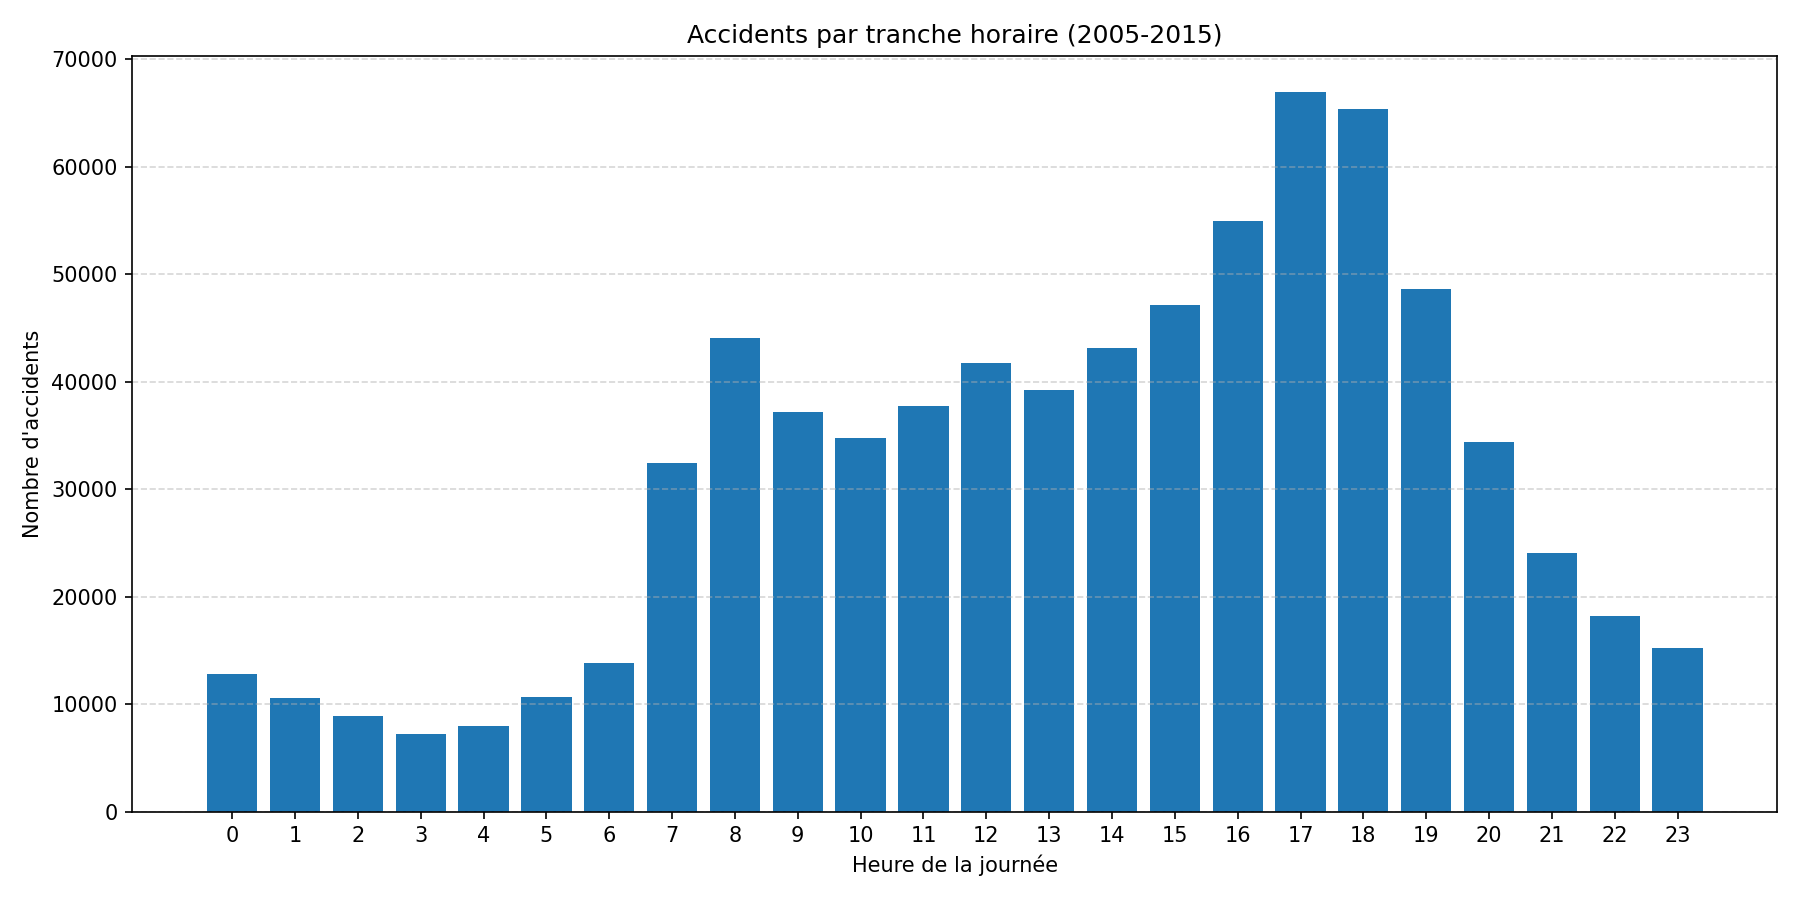
\includegraphics[width=0.85\linewidth]{../results/reponse61.png}
\caption{Q6.1 — Nombre d'accidents par tranche horaire d'une heure (métropole, 2005-2015)}
\end{figure}

\begin{center}
\begin{tabular}{l r}
\hline
\textbf{Indicateur} & \textbf{Valeur} \\
\hline
Total accidents (métropole, 2005-2015) & 757 263 \\
Valeurs \texttt{hrmn} ignorées & 0 \\
Heure de pointe & \textbf{17h} (66 958 accidents) \\
Second pic & 18h (65 343) puis 8h (44 033) \\
Heure la plus calme & 3h (7 211 accidents) \\
Cumul nuit profonde (0h-5h) & 58 185 (≈ 7,7 \%) \\
\hline
\end{tabular}
\end{center}

\rub{labanalyse}{Vérifications réalisées + analyse.}

\begin{itemize}
\item \emph{Conservation du total} : la somme des 24 tranches (757 263) coïncide exactement avec le total des accidents métropolitains cumulés sur la période, et aucune valeur n'est perdue (0 ignorée). L'histogramme couvre bien les 24 heures.
\item \emph{Plausibilité de la forme} : la distribution est \textbf{bimodale} et épouse les déplacements domicile-travail — un pic le matin (8h, 44 033) et un pic plus marqué le soir (17h-18h, ≈ 66 000), un creux la nuit (minimum à 3h, 7 211). Ce profil est conforme à ce qu'on attend du trafic routier et constitue un test de cohérence du traitement.
\item \emph{Robustesse de l'extraction} : un contrôle sur des valeurs courtes (« 300 », « 30 ») confirme que \texttt{int(hrmn) // 100} les classe correctement (3h et 0h), là où un découpage de chaîne aurait produit des heures aberrantes.
\end{itemize}

\rub{labcomment}{Commentaires.} Le graphique met en évidence que les accidents ne sont pas répartis uniformément dans la journée : ils suivent l'intensité du trafic. Le pic du soir (17h-18h) dépasse celui du matin, ce qui s'explique classiquement par un trafic de retour plus étalé, une fatigue de fin de journée et une luminosité déclinante en partie de l'année. Les heures nocturnes (0h-5h) concentrent peu d'accidents en valeur absolue (≈ 7,7 \% du total) — mais ce volume faible ne préjuge pas de leur gravité, qui sera examinée dans les questions suivantes.

\clearpage
\subsubsection*{Question 6.2 — Tués cumulés par tranche d'âge et sexe}
\addcontentsline{toc}{subsubsection}{Question 6.2 — Tués cumulés par tranche d'âge et sexe}

\rub{labrappel}{Rappel de la question.} Fournir un graphique présentant le nombre de tués cumulé sur la période du projet par tranche d'âge (de 5 années) et par sexe.

\begin{agentbox}
\begin{itemize}
\item \textbf{Contexte} : table \emph{usagers} (\texttt{data/enriched/}), cumul 2005-2015. Tué = \texttt{grav == "2 - Tué"}, sexe lu sur \texttt{sexe} (« 1 - Masculin » / « 2 - Féminin »).
\item \textbf{Décisions} : âge = \texttt{annee\_fichier - an\_nais} (millésimes complets à 4 chiffres, pas de reconstruction du siècle) ; \texttt{an\_nais} vide, « 0 » ou donnant un âge hors \textbf{[0, 120]} ignorée (96 cas, 0,2 \%). Métropole : la table \emph{usagers} ne porte pas le département → jointure sur \emph{caractéristiques} (\texttt{Num\_Acc} + \texttt{normaliser\_dep}), comme en Q2.
\item \textbf{Graphique} : 19 tranches de 5 ans (\texttt{0-4 … 85-89} + \texttt{90+} ouverte), \textbf{barres groupées} H/F, rendu matplotlib hors écran.
\end{itemize}
\end{agentbox}

\rub{labfichier}{Fichier Python :} \texttt{python/question62.py}.

\rub{labverif}{Vérification (pandas)} --- \texttt{python/verification62.py} → \texttt{results/verification62.txt} :

\begin{lstlisting}[style=pyblock]
>>> tues = usagers[(usagers.grav == "2 - Tué") & metropole]
>>> recap = tues.groupby([tranche_age, "sexe"]).size()
>>> recap          # extrait : 8 premieres tranches

tranche  hommes  femmes
    0-4     223     174
    5-9     191     159
  10-14     313     190
  15-19    3145     860
  20-24    5601    1176
  25-29    4015     694
  30-34    2863     513
  35-39    2516     511

# conforme : effectifs identiques a question62.py (H=33921, F=10899)
\end{lstlisting}

\rub{labresultat}{Résultat :} \texttt{results/reponse62.png} — barres groupées (axe x = tranche d'âge, 2 barres par tranche, axe y = nombre de tués cumulés), titre « Tués cumulés par tranche d'âge et par sexe (2005-2015) », taille 14×7 pouces. Bilan sur \textbf{44 820} tués métropolitains :

\begin{figure}[h]
\centering
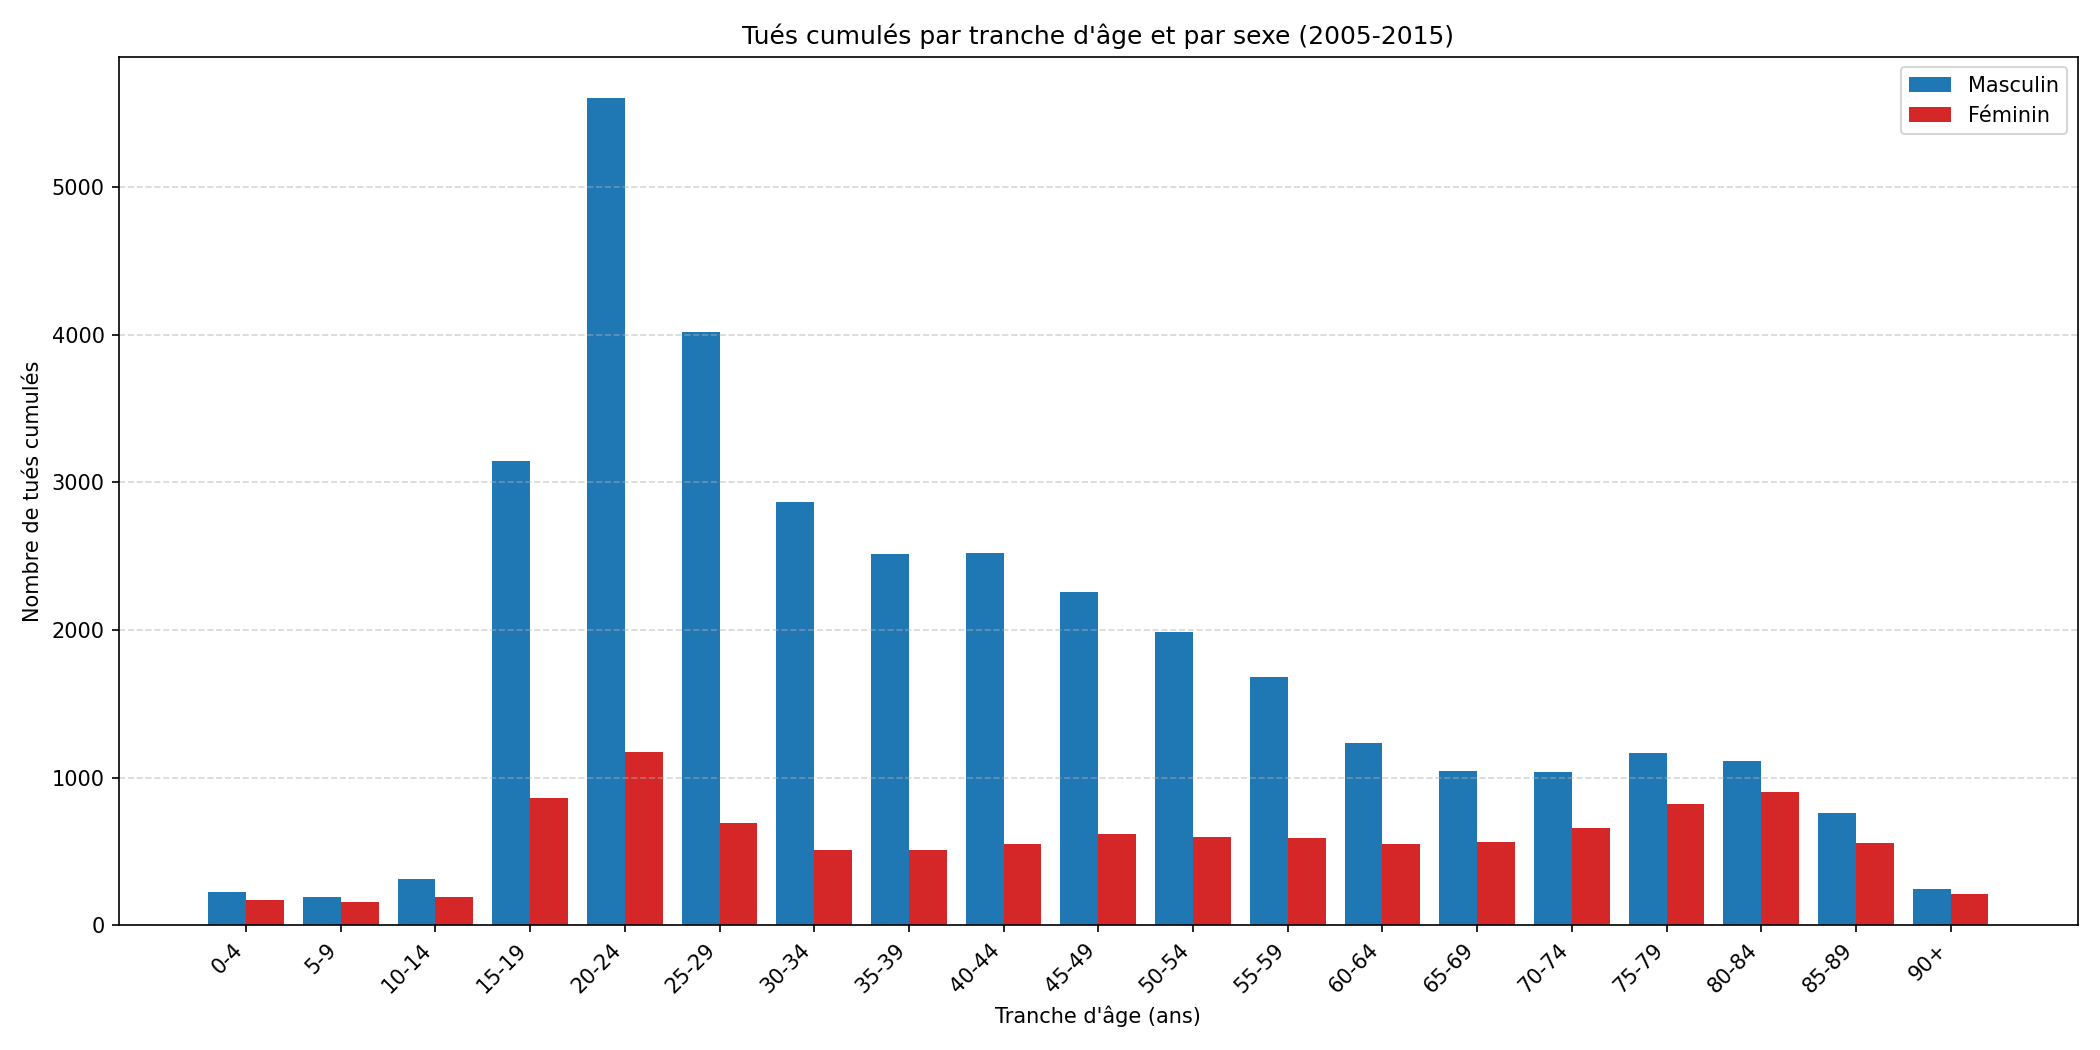
\includegraphics[width=0.85\linewidth]{../results/reponse62.png}
\caption{Q6.2 — Tués cumulés par tranche d'âge (5 ans) et par sexe (métropole, 2005-2015)}
\end{figure}

\begin{center}
\begin{tabular}{l r}
\hline
\textbf{Indicateur} & \textbf{Valeur} \\
\hline
Total tués (métropole, 2005-2015) & 44 820 \\
dont hommes & 33 921 (75,7 \%) \\
dont femmes & 10 899 (24,3 \%) \\
Tranche la plus touchée & \textbf{20-24 ans} (6 777 tués) \\
Tués au sexe non renseigné & 0 \\
Tués à l'âge non exploitable (ignorés) & 96 \\
\hline
\end{tabular}
\end{center}

\rub{labanalyse}{Vérifications réalisées + analyse.}

\begin{itemize}
\item \emph{Conservation des effectifs} : la somme hommes + femmes des 19 tranches (44 820) coïncide avec le cumul des tués métropolitains affiché année par année, et le sexe est intégralement renseigné chez les tués (0 ignoré). Seuls 96 tués (0,2 \%) sont écartés faute d'âge exploitable.
\item \emph{Plausibilité de la forme} : la distribution présente un \textbf{pic marqué sur les 20-24 ans} (6 777 tués) puis 15-19 et 25-29, conforme à la surmortalité routière bien documentée des jeunes adultes (prise de risque, inexpérience), avant une décroissance régulière avec l'âge.
\item \emph{Plausibilité de l'écart hommes/femmes} : les hommes représentent \textbf{75,7 \%} des tués, un déséquilibre constant sur toutes les tranches et cohérent avec les statistiques nationales de la sécurité routière (exposition au volant et profils de conduite). Un léger resserrement de l'écart apparaît aux âges élevés.
\end{itemize}

\rub{labcomment}{Commentaires.} Le graphique croise deux facteurs de risque — l'âge et le sexe — et fait ressortir une population particulièrement exposée : les \textbf{hommes jeunes (15-29 ans)}, qui concentrent à eux seuls une part majeure des tués. La tranche \texttt{90+}, ouverte, reste résiduelle en valeur absolue. Ce résultat éclaire les questions de gravité : au-delà du volume d'accidents (Q6.1), c'est ici la mortalité qui est ventilée, et elle ne suit pas la même structure démographique que l'ensemble des usagers impliqués.

\clearpage
\subsubsection*{Question 6.3 — Top 10 départements (carte folium)}
\addcontentsline{toc}{subsubsection}{Question 6.3 — Top 10 départements (carte folium)}

\rub{labrappel}{Rappel de la question.} Quels sont les 10 départements avec le plus d'accidents ? L'affichage se fait sur une carte de France en utilisant la bibliothèque \textbf{folium}.

\begin{agentbox}
\begin{itemize}
\item \textbf{Contexte} : table \emph{caractéristiques} (\texttt{data/enriched/}), cumul 2005-2015 ; 1 ligne = 1 accident, donc décompte par département par simple comptage (\texttt{collections.Counter}), sans jointure.
\item \textbf{Décision (département)} : \texttt{dep} est codé \texttt{département × 10} (Paris \texttt{750}, Nord \texttt{590}), repassé au code INSEE via \texttt{normaliser\_dep}, qui gère la Corse (\texttt{201 → 2A}, \texttt{202 → 2B}) et \textbf{exclut DOM / non-métropole} (\texttt{None}).
\item \textbf{Carte folium} : top 10 en \textbf{cercles rouges proportionnels} (popup + tooltip), tous les autres départements en petits marqueurs gris discrets ; fond \texttt{CartoDB positron}, centrage \texttt{(46.5, 2.0)}, zoom 6.
\end{itemize}
\end{agentbox}

\rub{labfichier}{Fichier Python :} \texttt{python/question63.py}.

\rub{labverif}{Vérification (pandas)} --- \texttt{python/verification63.py} → \texttt{results/verification63.txt} :

\begin{lstlisting}[style=pyblock]
>>> recap = (caracteristiques["dep"].map(normaliser_dep)
...               .value_counts().head(10))
>>> recap          # top 10 departements

 rang dep  accidents
    1  75      81016
    2  13      48078
    3  93      30779
    4  92      28388
    5  06      27038
    6  94      26668
    7  69      23658
    8  59      22657
    9  33      20813
   10  91      16044

# conforme : meme top 10 (departement + effectif) que reponse63.txt
\end{lstlisting}

\rub{labresultat}{Résultat :} \texttt{results/reponse63.html} (carte interactive) et \texttt{results/reponse63.txt} (tableau). Sur \textbf{757 263} accidents métropolitains cumulés répartis sur 96 départements, le classement est :

\begin{figure}[h]
\centering
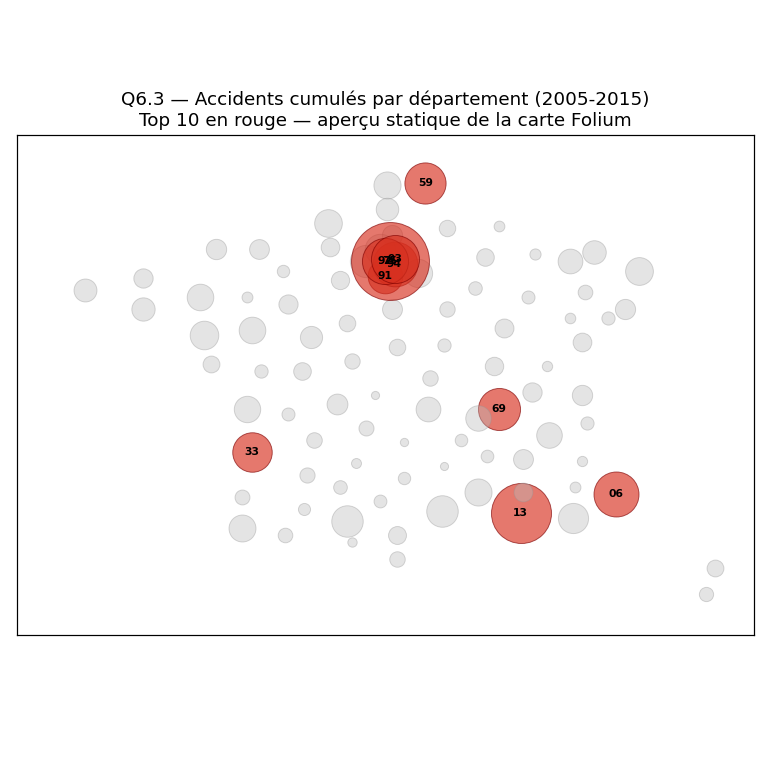
\includegraphics[width=0.85\linewidth]{../results/reponse63_apercu.png}
\caption{Q6.3 — Aperçu statique de la carte Folium : accidents cumulés par département, top 10 en rouge (métropole, 2005-2015). La carte interactive est dans \texttt{results/reponse63.html}.}
\end{figure}

\begin{center}
\begin{tabular}{r c l r}
\hline
\textbf{Rang} & \textbf{Dép.} & \textbf{Nom} & \textbf{Nb accidents} \\
\hline
1 & 75 & Paris & 81 016 \\
2 & 13 & Bouches-du-Rhône & 48 078 \\
3 & 93 & Seine-Saint-Denis & 30 779 \\
4 & 92 & Hauts-de-Seine & 28 388 \\
5 & 06 & Alpes-Maritimes & 27 038 \\
6 & 94 & Val-de-Marne & 26 668 \\
7 & 69 & Rhône & 23 658 \\
8 & 59 & Nord & 22 657 \\
9 & 33 & Gironde & 20 813 \\
10 & 91 & Essonne & 16 044 \\
\hline
\end{tabular}
\end{center}

\rub{labanalyse}{Vérifications réalisées + analyse.}

\begin{itemize}
\item \emph{Conservation des effectifs} : la somme des comptes par département (757 263) coïncide avec le cumul affiché année par année par le script, et le nombre de départements représentés (\textbf{96} = 95 + Corse \texttt{2A}/\texttt{2B}) confirme que le \texttt{20} corse a bien été éclaté et qu'aucun DOM n'est compté.
\item \emph{Plausibilité géographique} : le top 10 est dominé par \textbf{Paris et la petite couronne} (75, 93, 92, 94) plus les grandes métropoles (Bouches-du-Rhône/Marseille, Alpes-Maritimes/Nice, Rhône/Lyon, Nord/Lille, Gironde/Bordeaux) — résultat attendu, le nombre d'accidents suivant la densité de population et de trafic urbain. Paris domine très nettement (81 016, soit \textasciitilde{}1,7× le 2ᵉ).
\item \emph{Vérification de la carte} : ouverture du \texttt{.html}, contrôle visuel du placement des cercles sur les bons départements, de la proportionnalité des rayons (Paris le plus gros), et du contenu des popups (nom + effectif).
\end{itemize}

\rub{labcomment}{Commentaires.} Le décompte est \textbf{brut} (volume d'accidents), non rapporté à la population ou au trafic : il mesure donc l'exposition absolue, pas un risque par habitant. Les départements urbains denses ressortent logiquement en tête. Une normalisation (accidents pour 100 000 habitants ou par véhicule-km) donnerait un classement très différent et ferait remonter des départements ruraux ou de transit — piste possible pour la question libre Q6.4.

\clearpage
\subsubsection*{Question 6.4 — Question libre}
\addcontentsline{toc}{subsubsection}{Question 6.4 — Question libre}

\rub{labrappel}{Rappel de la question.} Question libre à définir, utilisant \textbf{au moins deux types de table} (parmi \emph{caractéristiques}, \emph{lieux}, \emph{véhicules}, \emph{usagers}) et \textbf{un type d'affichage non utilisé précédemment} (camembert exclu).

*\emph{Question retenue : }Comment les accidents se répartissent-ils selon les conditions atmosphériques (\texttt{atm}) croisées avec l'état de la surface de la route (\texttt{surf}) ?**\emph{ Les deux variables sont }a priori* corrélées (la pluie mouille la chaussée, la neige l'enneige) mais pas confondues — on attend des cellules « hors diagonale » instructives (pluie sur chaussée déjà verglacée, temps normal sur chaussée mouillée résiduelle, etc.).

\begin{agentbox}
\begin{itemize}
\item \textbf{Tables (contrainte ≥ 2)} : \texttt{atm} (\emph{caractéristiques}) × \texttt{surf} (\emph{lieux}), jointes par \texttt{Num\_Acc} ; filtrage métropole dès la première table (\texttt{normaliser\_dep}) pour ne nourrir la matrice que d'accidents métropolitains.
\item \textbf{Affichage (inédit, camembert exclu)} : \textbf{heatmap} \texttt{atm} × \texttt{surf} via \texttt{matplotlib.imshow} (\texttt{seaborn} hors dépendances), cellules annotées. Échelle \textbf{logarithmique} (\texttt{LogNorm}) car (\texttt{Normale}, \texttt{Normale}) écrase tout (76 \%) — sinon toute la grille apparaît uniforme.
\item \textbf{Détails} : libellés \textbf{abrégés aux deux premiers mots} (un seul provoquait des collisions « Pluie légère »/« forte ») ; \texttt{atm} vide (21) et \texttt{surf} vide ou \texttt{0} (23 375) ignorés ; modalités figées dans l'ordre du référentiel.
\end{itemize}
\end{agentbox}

\rub{labfichier}{Fichier Python :} \texttt{python/question64.py}.

\rub{labverif}{Vérification (pandas)} --- \texttt{python/verification64.py} → \texttt{results/verification64.txt} :

\begin{lstlisting}[style=pyblock]
>>> f = lieux.merge(carac_metropole, on="Num_Acc")
>>> recap = f.groupby(["atm","surf"]).size()
>>> recap          # totaux exploites / ignores / couple dominant

           controle  pandas
accidents_exploites  733867
        atm_ignores      21
       surf_ignores   23375
top_couple_effectif  560189

# conforme : identiques a reponse64.txt ; couple dominant 1 - Normale x 1 - Normale
\end{lstlisting}

\rub{labresultat}{Résultat :} \texttt{results/reponse64.png} (heatmap) et \texttt{results/reponse64.txt} (trace). Sur \textbf{733 867} accidents métropolitains exploitables (cumul 2005-2015), les couples les plus fréquents sont :

\begin{figure}[h]
\centering
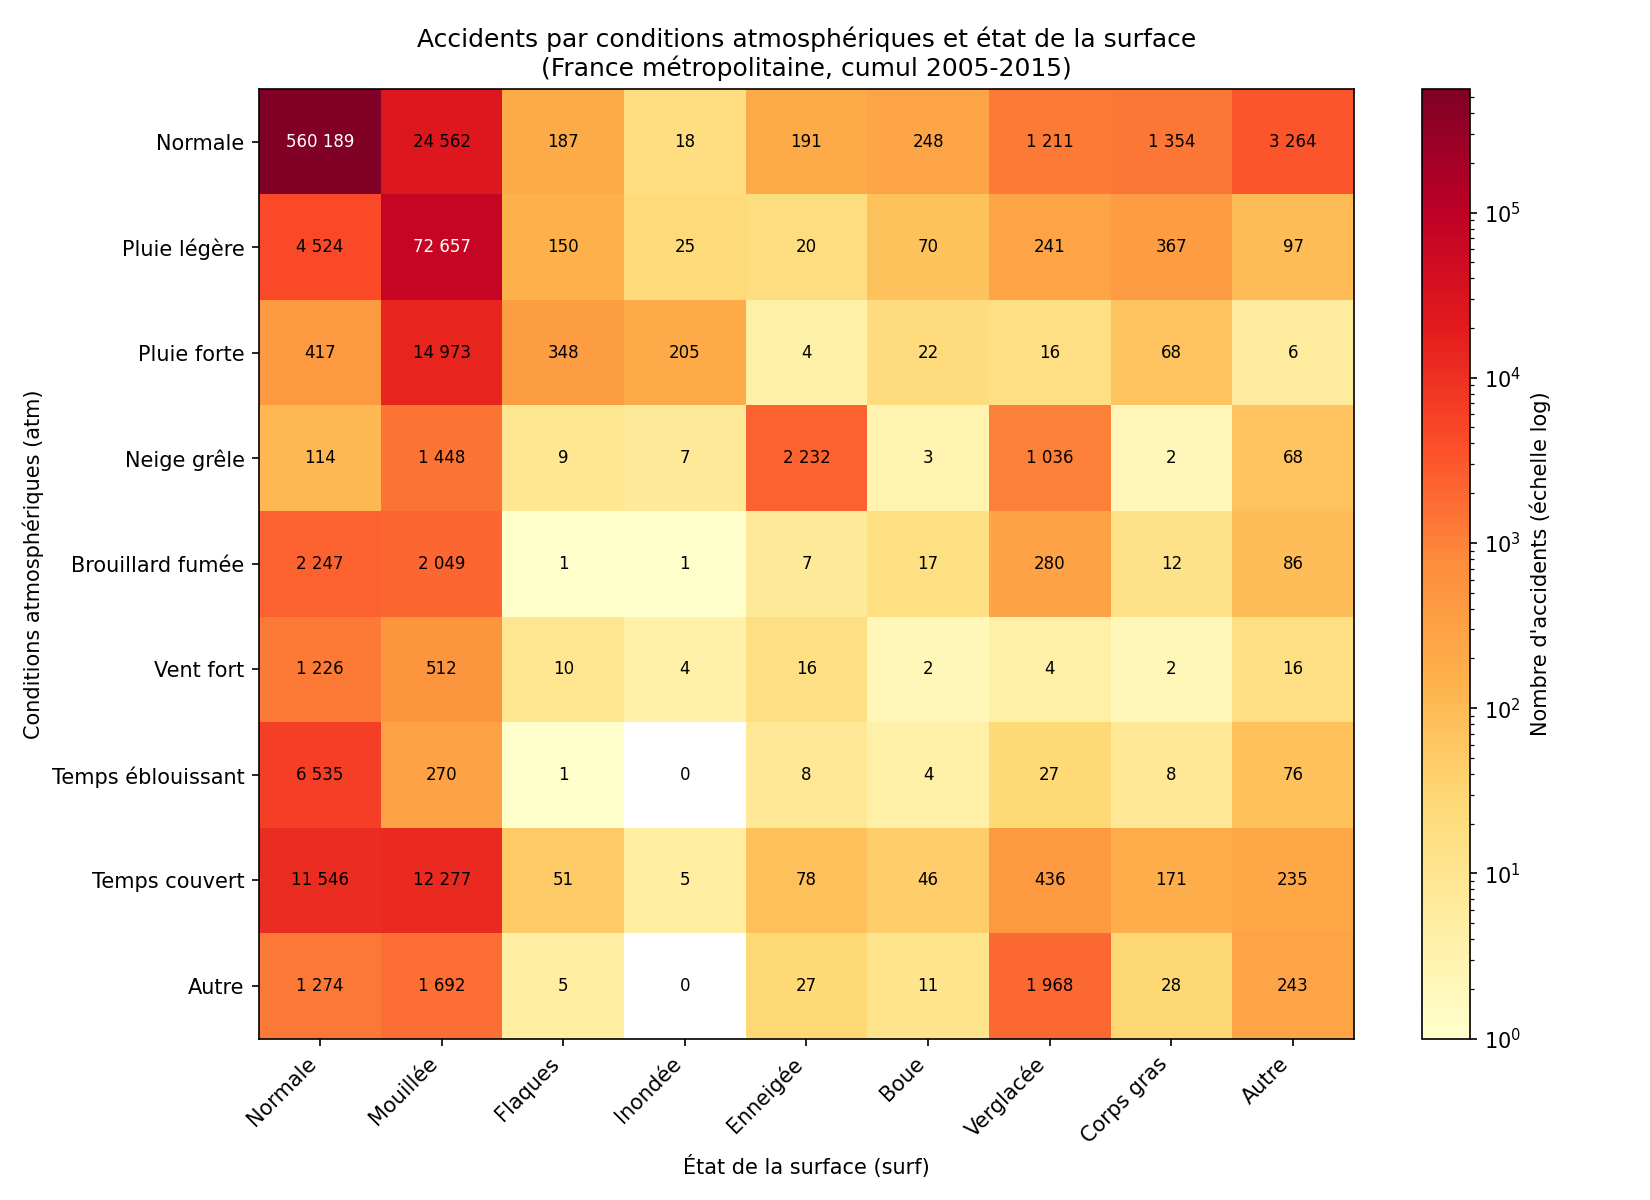
\includegraphics[width=0.85\linewidth]{../results/reponse64.png}
\caption{Q6.4 — Heatmap des accidents selon les conditions atmosphériques (\texttt{atm}) × état de la surface (\texttt{surf}), échelle logarithmique (métropole, 2005-2015)}
\end{figure}

\begin{center}
\begin{tabular}{l l r r}
\hline
\textbf{Conditions atm.} & \textbf{État surface} & \textbf{Nb accidents} & \textbf{Part} \\
\hline
Normale & Normale & 560 189 & 76,3 \% \\
Pluie légère & Mouillée & 72 657 & 9,9 \% \\
Normale & Mouillée & 24 562 & 3,3 \% \\
Pluie forte & Mouillée & 14 973 & 2,0 \% \\
Temps couvert & Mouillée & 12 277 & 1,7 \% \\
\hline
\end{tabular}
\end{center}

\rub{labanalyse}{Vérifications réalisées + analyse.}

\begin{itemize}
\item \emph{Conservation des effectifs} : le total exploité (733 867) = total métropolitain de Q6.3 (757 263) − les 23 396 accidents écartés pour \texttt{atm}/\texttt{surf} non renseignés (21 + 23 375). Cohérent.
\item \emph{Cohérence physique de la diagonale} : les cellules attendues ressortent nettement — \textbf{pluie légère × mouillée} (72 657, 2ᵉ couple), \textbf{neige-grêle × enneigée} (2 232), \textbf{temps couvert/pluie × mouillée}. Le verglas apparaît surtout sur \texttt{Neige grêle × Verglacée} (1 036) et \texttt{Autre × Verglacée} (1 968, le « Autre » atmosphérique recouvrant vraisemblablement le grand froid sec).
\item \emph{Cellules hors diagonale instructives} : \textbf{6 535 accidents par temps éblouissant sur chaussée normale} (l'éblouissement n'altère pas la route mais la visibilité), et \textbf{24 562 accidents en temps « Normale » sur chaussée mouillée} (chaussée encore humide après la pluie alors que le ciel est redevenu clair) — ces deux poches justifient le croisement plutôt que deux histogrammes séparés.
\item \emph{Contrôle visuel} : ouverture du PNG, vérification que les libellés d'axes sont distincts, que l'échelle log rend les modalités rares visibles, et que les annotations chiffrées correspondent à la trace texte.
\end{itemize}

\rub{labcomment}{Commentaires.} L'écrasante domination de (\texttt{Normale}, \texttt{Normale}) reflète simplement le fait que la plupart des trajets se font par beau temps sur route sèche : la heatmap mesure des \textbf{volumes}, pas un sur-risque. Pour en déduire un risque relatif il faudrait rapporter chaque cellule à l'exposition (temps passé dans chaque condition météo/surface), donnée absente du BAAC. La lecture pertinente est donc \textbf{comparative entre conditions dégradées} : à conditions rares, la chaussée mouillée concentre l'essentiel des accidents pluvieux, et l'enneigement/verglas forme un bloc cohérent neige↔surface, ce qui valide la qualité du croisement des deux tables.

\clearpage
\subsubsection*{Question 6.5 \emph{(facultative)} — Carte animée par année}
\addcontentsline{toc}{subsubsection}{Question 6.5 \emph{(facultative)} — Carte animée par année}

\rub{labrappel}{Rappel de la question.} Reprendre la question 6.3 et en faire un \textbf{GIF animé} de la carte, \textbf{année par année}.

\begin{agentbox}
\begin{itemize}
\item \textbf{Bibliothèque} : folium produit du HTML, inadapté à un GIF → chaque frame tracée en \textbf{matplotlib} (\texttt{Agg}) puis les 11 PNG empilés en GIF avec \textbf{Pillow} (\texttt{duration=800, loop=0}). Dépendances déjà présentes (Pillow tiré par matplotlib).
\item \textbf{Tracé} : départements placés à leur \textbf{centroïde} (\texttt{CENTROIDES\_DEPARTEMENTS}) ; \texttt{x=lon, y=lat} + \texttt{set\_aspect("equal")} reconstitue la silhouette de l'Hexagone sans frontières. Cadre fixe (lon −5,5→10, lat 41→51,5), aire \texttt{s} de \texttt{scatter} ∝ effectif.
\item \textbf{Décision clé (échelle comparable)} : normaliser les rayons année par année masquerait l'évolution ; on calcule donc le \textbf{maximum global} (Paris 2005, \textbf{8 591} accidents) et on y rapporte tous les cercles, qui rétrécissent visiblement de 2005 à 2015. PNG intermédiaires supprimés après assemblage.
\end{itemize}
\end{agentbox}

\rub{labfichier}{Fichier Python :} \texttt{python/question65.py}.

\rub{labverif}{Vérification (pandas)} --- \texttt{python/verification65.py} → \texttt{results/verification65.txt} :

\begin{lstlisting}[style=pyblock]
>>> recap = (caracteristiques["dep"].map(normaliser_dep)
...               .value_counts())          # par annee
>>> recap          # nb departements + total metropole / annee

 annee  departements  total_metropole
  2005            96            84525
  2006            96            80309
  2007            96            81272
  2008            96            74487
  2009            96            72315
  2010            96            67288
  2011            96            65024
  2012            96            60437
  2013            96            56812
  2014            96            58191
  2015            96            56603

# conforme : comptes par departement identiques annee par annee
\end{lstlisting}

\rub{labresultat}{Résultat :} \texttt{results/reponse65.gif} — animation de \textbf{11 images} (2005→2015), 600×600 px, 800 ms par image, boucle infinie. Le décompte métropolitain par année décroît régulièrement :

\begin{figure}[h]
\centering
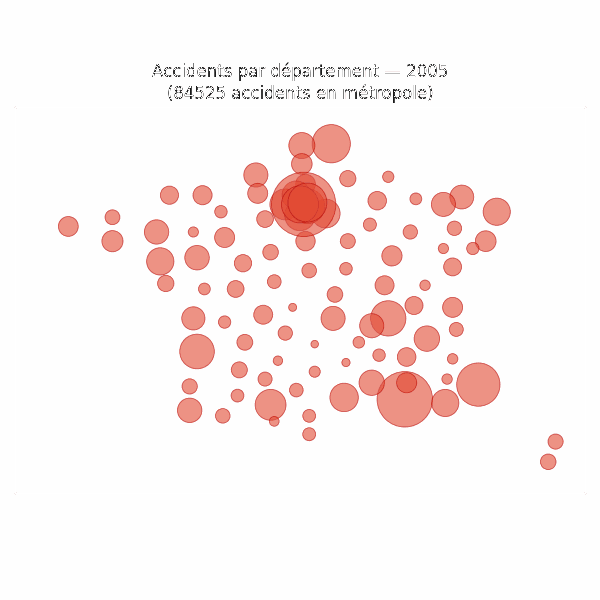
\includegraphics[width=0.85\linewidth]{../results/reponse65_frame.png}
\caption{Q6.5 — Première image (2005) du GIF animé \texttt{results/reponse65.gif} : accidents par département, cercles proportionnels (métropole)}
\end{figure}

\begin{center}
\begin{tabular}{r r l r r}
\hline
\textbf{Année} & \textbf{Accidents métropole} & \textbf{} & \textbf{Année} & \textbf{Accidents métropole} \\
\hline
2005 & 84 525 &  & 2011 & 65 024 \\
2006 & 80 309 &  & 2012 & 60 437 \\
2007 & 81 272 &  & 2013 & 56 812 \\
2008 & 74 487 &  & 2014 & 58 191 \\
2009 & 72 315 &  & 2015 & 56 603 \\
2010 & 67 288 &  &  &  \\
\hline
\end{tabular}
\end{center}

\rub{labanalyse}{Vérifications réalisées + analyse.}

\begin{itemize}
\item \emph{Conservation des effectifs} : la somme des 11 totaux annuels (757 263) coïncide avec le cumul métropolitain de Q6.3, et chaque total annuel est réaffiché par le script — aucune ligne perdue ni dupliquée.
\item \emph{Structure du GIF} : relecture du fichier avec Pillow → \texttt{n\_frames = 11}, \texttt{duration = 800}, \texttt{loop = 0}, taille 600×600 ; les 11 PNG temporaires ont bien disparu du dossier \texttt{results/}.
\item \emph{Contrôle visuel} : ouverture de la première (2005) et de la dernière (2015) frame. La silhouette de la France est reconnaissable, \textbf{Paris} (75) forme le gros amas sombre central, la \textbf{Corse} apparaît détachée en bas à droite, et les cercles \textbf{rétrécissent nettement} entre 2005 et 2015 — l'animation traduit donc bien la baisse continue des accidents.
\end{itemize}

\rub{labcomment}{Commentaires.} L'animation met en évidence la \textbf{baisse tendancielle} du nombre d'accidents corporels sur la décennie (−33 \% entre 2005 et 2015), cohérente avec le renforcement des politiques de sécurité routière. La représentation reste \textbf{volumétrique} (mêmes réserves qu'en Q6.3 : pas de normalisation par population/trafic) et \textbf{schématique} (centroïdes plutôt qu'un vrai fond cartographique) : son intérêt est la lecture dynamique de l'évolution, pas la précision géographique. Un fond \texttt{geopandas}/contours départementaux donnerait un rendu choroplèthe plus fin, au prix d'une dépendance supplémentaire non requise par le sujet.

\section*{Conclusion / synthèse}
\addcontentsline{toc}{section}{Conclusion / synthèse}

\textbf{Qualité des données.} L'intégrité référentielle du jeu BAAC 2005-2015 (Groupe 1) est globalement très bonne. Le lien \emph{usager → véhicule} est quasi parfait (22 violations sur 1 742 583 usagers, soit 0,0013 \%), et le lien inverse \emph{véhicule → usager} ne présente que 1,47 \% de véhicules sans usager (19 580 cas), majoritairement explicables par les conducteurs en fuite. Les contrôles facultatifs \emph{lieu ↔ accident} (Q2.3) et \emph{accident → lieu unique} (Q2.4) confirment cette cohérence. Le seul attribut véritablement fragile au sens de la saisie est le sens de circulation (\texttt{senc}) ; les taux d'absence élevés de \texttt{obs}/\texttt{obsm}/\texttt{choc}/\texttt{occutc} (Q4.1) traduisent surtout des « sans objet » légitimes (code \texttt{0}) et non des défauts de remplissage.

\textbf{Cohérence inter-attributs.} Les incohérences logiques recherchées (Q5) restent marginales : luminosité × heure (Q5.1), obstacle mobile × point de choc (Q5.2) et années de naissance impossibles (Q5.3, 41 cas sur 1,74 M) ne remettent pas en cause l'exploitabilité du jeu. Ces contrôles valident la fiabilité d'ensemble plus qu'ils ne révèlent des anomalies massives.

\textbf{Enseignements analytiques.} Les visualisations (Q6) dégagent des structures conformes aux connaissances de la sécurité routière : distribution horaire bimodale calée sur les déplacements domicile-travail (pic 17h-18h), surmortalité des hommes jeunes (15-29 ans, 75,7 \% des tués), concentration des accidents dans les départements urbains denses (Paris ≈ 1,7× le 2ᵉ), et baisse tendancielle de −33 \% du nombre d'accidents corporels entre 2005 et 2015.

\textbf{Limites.} Tous les décomptes géographiques et temporels sont \textbf{volumétriques} : ils mesurent une exposition absolue, non un risque rapporté à la population, au trafic ou aux véhicules-km — données absentes du BAAC. Les cartes (Q6.3/6.5) reposent sur des \textbf{centroïdes} départementaux, schématiques par rapport à un vrai fond cartographique.

\textbf{Pistes d'amélioration.} Normaliser les effectifs (accidents pour 100 000 habitants), enrichir avec un fond \texttt{geopandas} pour des cartes choroplèthes, et croiser gravité × infrastructure pour cibler les configurations les plus meurtrières.

\end{document}
